%%%%%%%%%%%%%%%%%%%%%%%%%%%%%%%%%%%%%%%%%%%%%%%%%%%%%%%%%
%%   $RCSfile: csli-hpsg-2003.tex,v $
%%  $Revision: 1.1 $
%%      $Date: 2003/10/12 13:42:57 $
%%     Author: Stefan Mueller (CL UNi Bremen)
%%    Purpose: 
%%   Language: LaTeX
%%%%%%%%%%%%%%%%%%%%%%%%%%%%%%%%%%%%%%%%%%%%%%%%%%%%%%%%%
%%
%% $Log: csli-hpsg-2003.tex,v $
%% Revision 1.1  2003/10/12 13:42:57  stefan
%% Initial revision
%%
%%%%%%%%%%%%%%%%%%%%%%%%%%%%%%%%%%%%%%%%%%%%%%%%%%%%%%%%%

\documentclass[11pt,a4paper,fleqn]{article}
\usepackage{times}
\thispagestyle{empty}



\usepackage[T1]{fontenc}   % Silbentrennung

\usepackage{8bit}

\usepackage[bookmarks=true,%
breaklinks=true,%
draft=false,colorlinks=false,plainpages=false,hyperfootnotes=false,%
linkcolor=black,%
pagecolor=black,%
pdfauthor={Stefan M�ller (Editor)},%
pdftitle={Proceedings of the HPSG03 Conference},%
pdfkeywords={HPSG}%,
pdftex=true%
%ps2pdf=true  %ohne diesen Treiber geht der Zeilenumbruch in URLs
]{hyperref}% for pdf files

\usepackage{pdfpages}

\hypersetup{colorlinks=false,linkcolor=black,pagecolor=black}

\begin{document}

\begin{center}
{\Large
                Proceedings of the HPSG03 Conference}\\[\baselineskip]

                Michigan State University, East Lansing\\[\baselineskip]

                        Stefan M{\"u}ller (Editor)\\[\baselineskip]

                                2003\\[\baselineskip]

                          CSLI Publications\\[\baselineskip]

              http://csli-publications.stanford.edu/

\end{center}
\newpage
\tableofcontents

\newpage

\section{Editor's Note}

The 10th International Conference on Head-driven Phrase Structure Grammar was held at
Michigan State University, Michigan in the USA. 

The conference featured three invited talks, 26 papers, and two alternate papers,
selected by the program committee 
(Bob Borsley, chair,
Doug Arnold,
Elisabet Engdahl,
Erhard Hinrichs,
Tom Hukari,
Andreas Kathol,
Jean-Pierre Koenig,
Shalom Lappin,
Detmar Meurers,
Tsuneko Nakazawa,
Adam Przepi�rkowski,
Ivan Sag,
Gert Webelhuth,
Sh�ichi Yatabe) with the help of additional reviewers (Ronnie Cann,
Dani�le Godard, 
Georgia Green,
Jeanette Gundel,
Caroline Heycock,
Ewan Klein,
Stefan M�ller,
Frank Richter,
Manfred Sailer, 
Andrew Spencer).
In total there were 42 submissions.
We want to thank the program committee and the external reviewers
for putting this nice conference program together.

Thanks go to Ivan Sag and Gert Webelhuth, who were in charge of local arrangements.
I also want to thank Ivan Sag for help regarding computational infrastructure in Stanford.

As was decided on the Business Meeting I will take care of editing the HPSG proceedings from now on,
in order to guarantee fast publication of the conference results
to make the work presented at the conference available to a wider audience. 
As in the past years the contributions to the conference proceedings are based on the five page abstract
that was reviewed by the program committee, but there is no additional reviewing of the
longer contribution to the proceedings.
To ensure easy access and fast publication we have chosen an electronic format.

The proceedings include all the papers except those by 
Olivier Bonami and Dani�le Godard,
Gosse Bouma,
Incheol Choi and Stephen Wechsler,
Robert Malouf,
Vanessa Metcalf,
Peter Sells,
and Kei Yoshimoto and Masahiro Kobayashi.


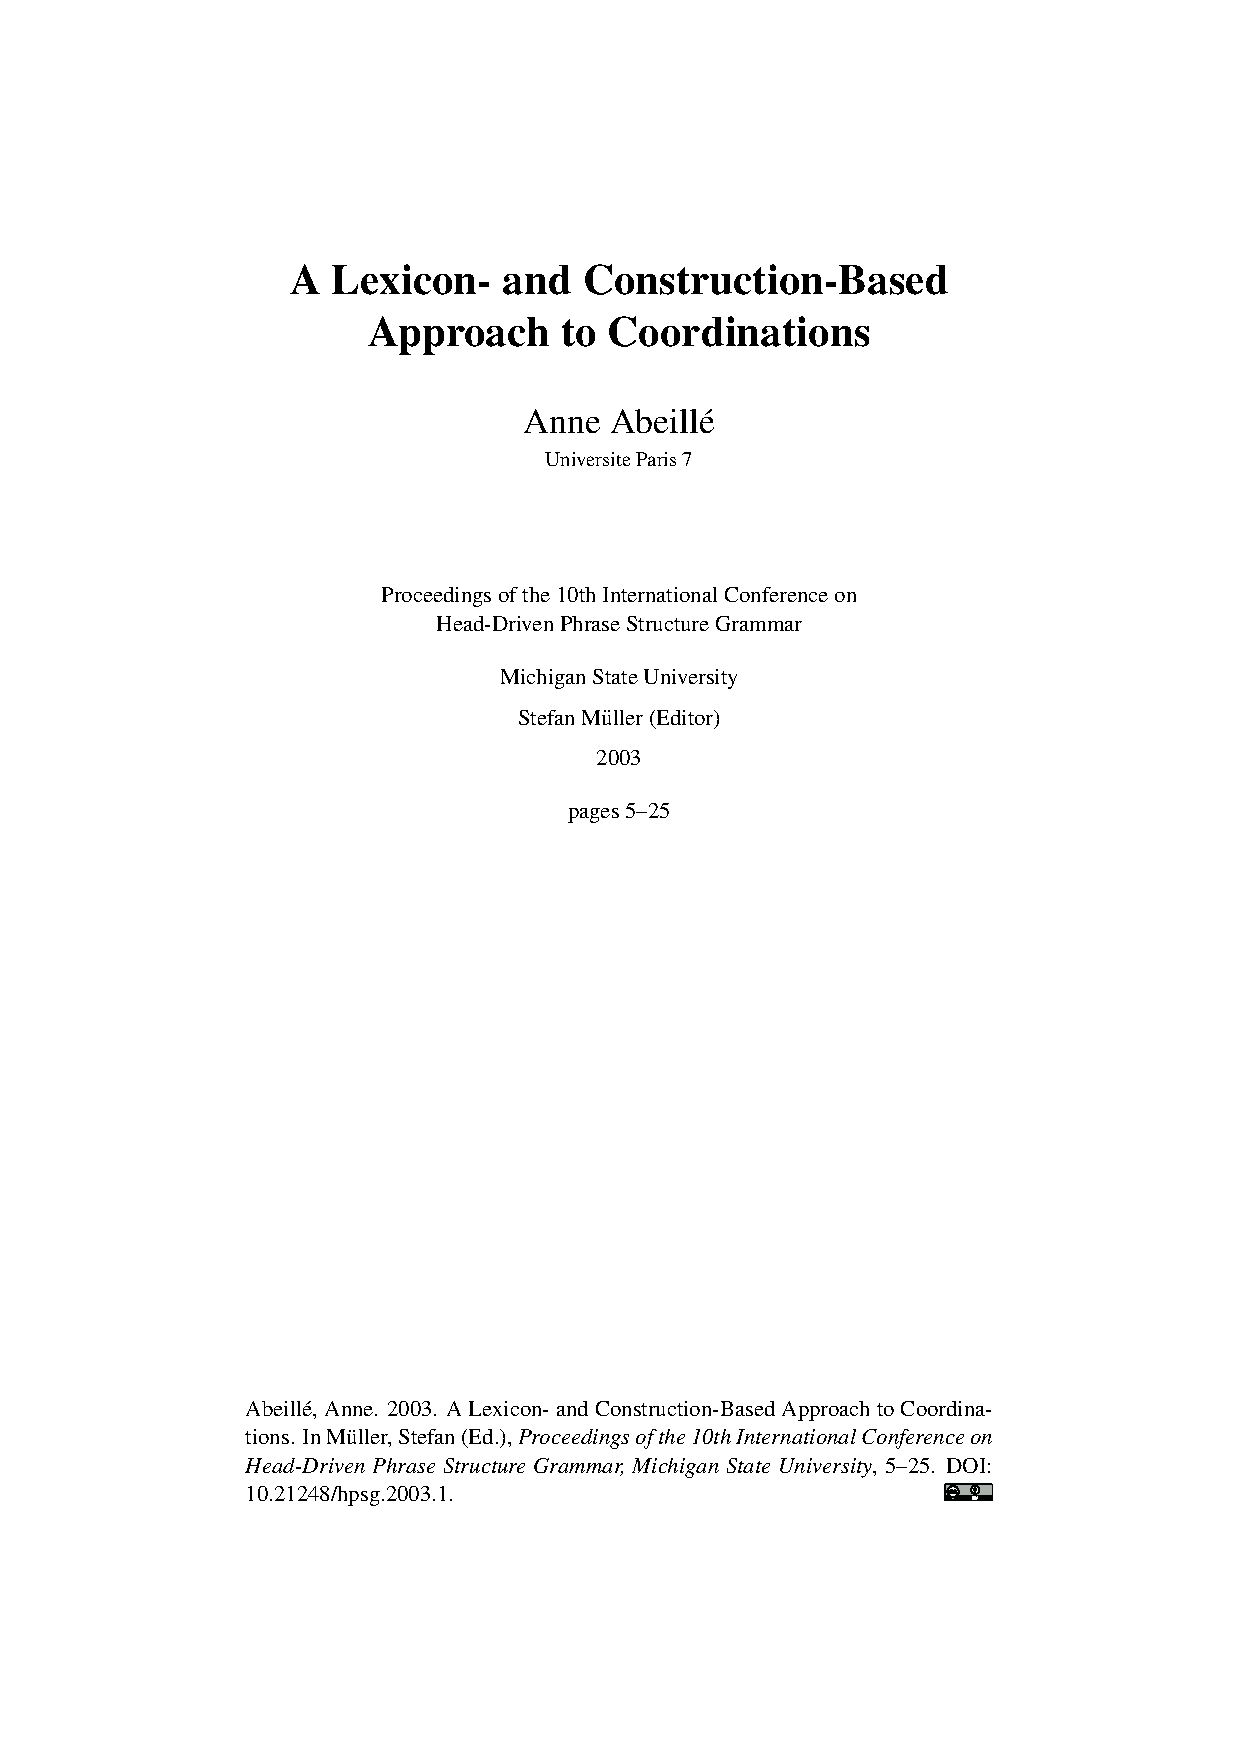
\includepdf[pages=-,pagecommand=\thispagestyle{plain},
           addtotoc={1,section,1,
                    {Anne Abeill�: A Lexicon- and Construction-Based Approach to Coordinations},
                    a}]{abeille.pdf}

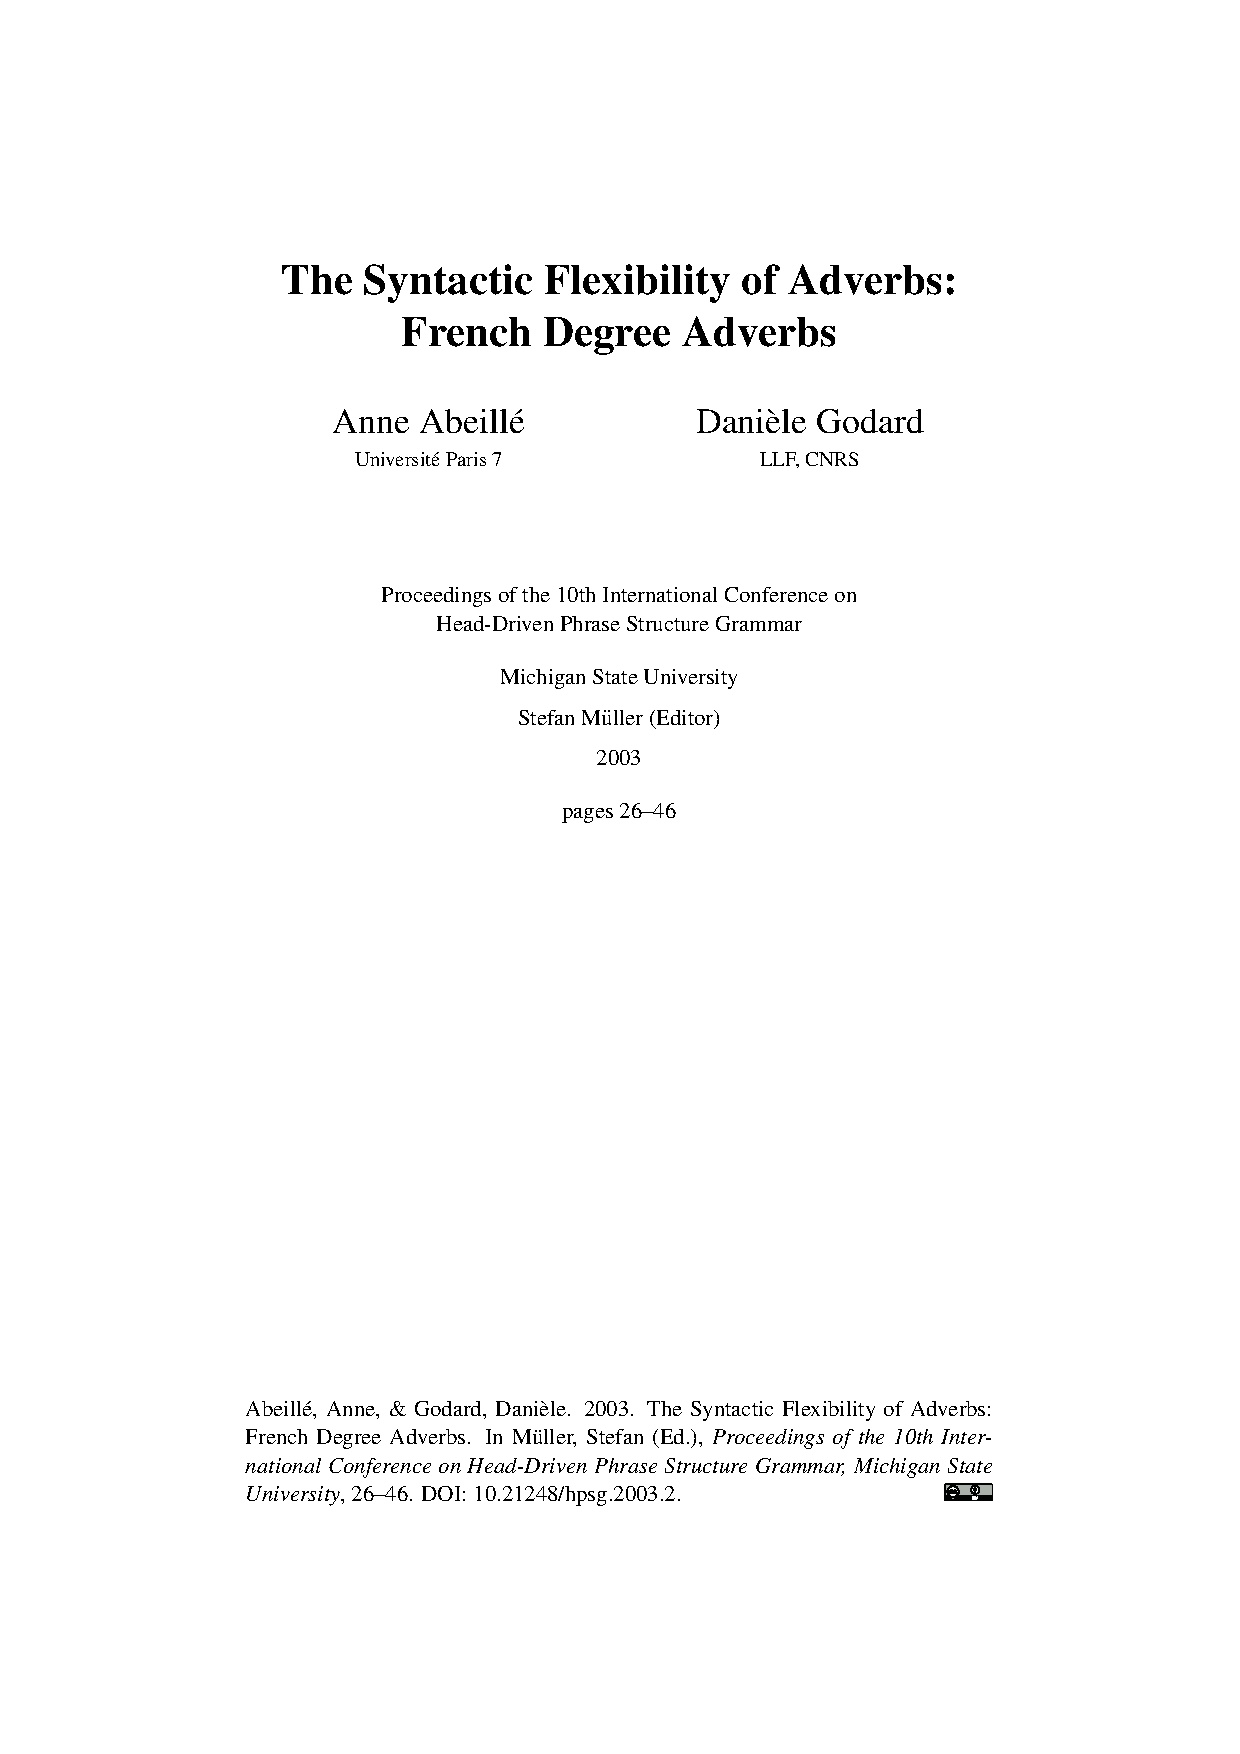
\includepdf[pages=-,pagecommand=\thispagestyle{plain},
           addtotoc={1,section,1,
                    {Anne Abeill� and Dani�le Godard: The Syntactic Flexibility of Adverbs: French Degree Adverbs},
                    ag}]{abeille-godard.pdf}

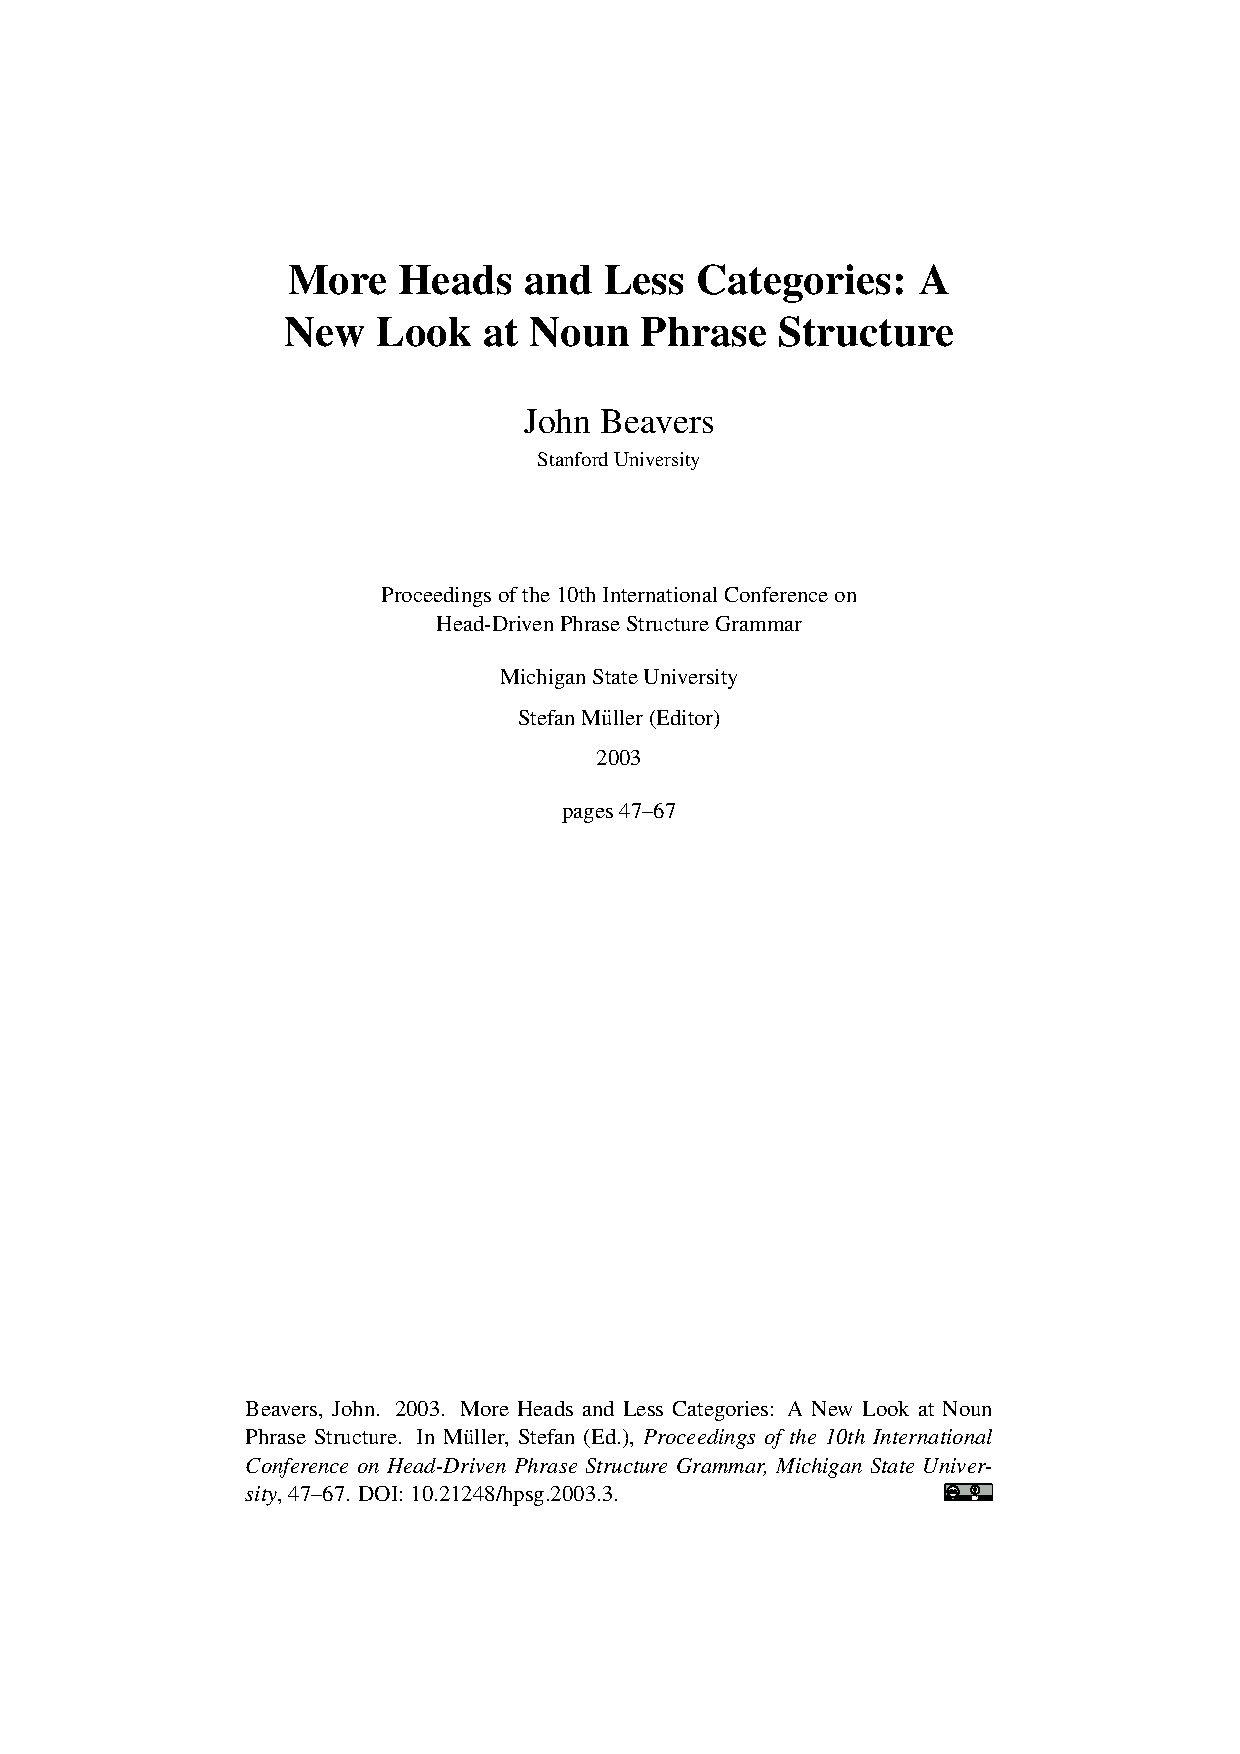
\includepdf[pages=-,pagecommand=\thispagestyle{plain},
           addtotoc={1,section,1,
                    {John Beavers: More Heads and Less Categories: A New Look at Noun Phrase Structure},
                    beavers}]{beavers.pdf}

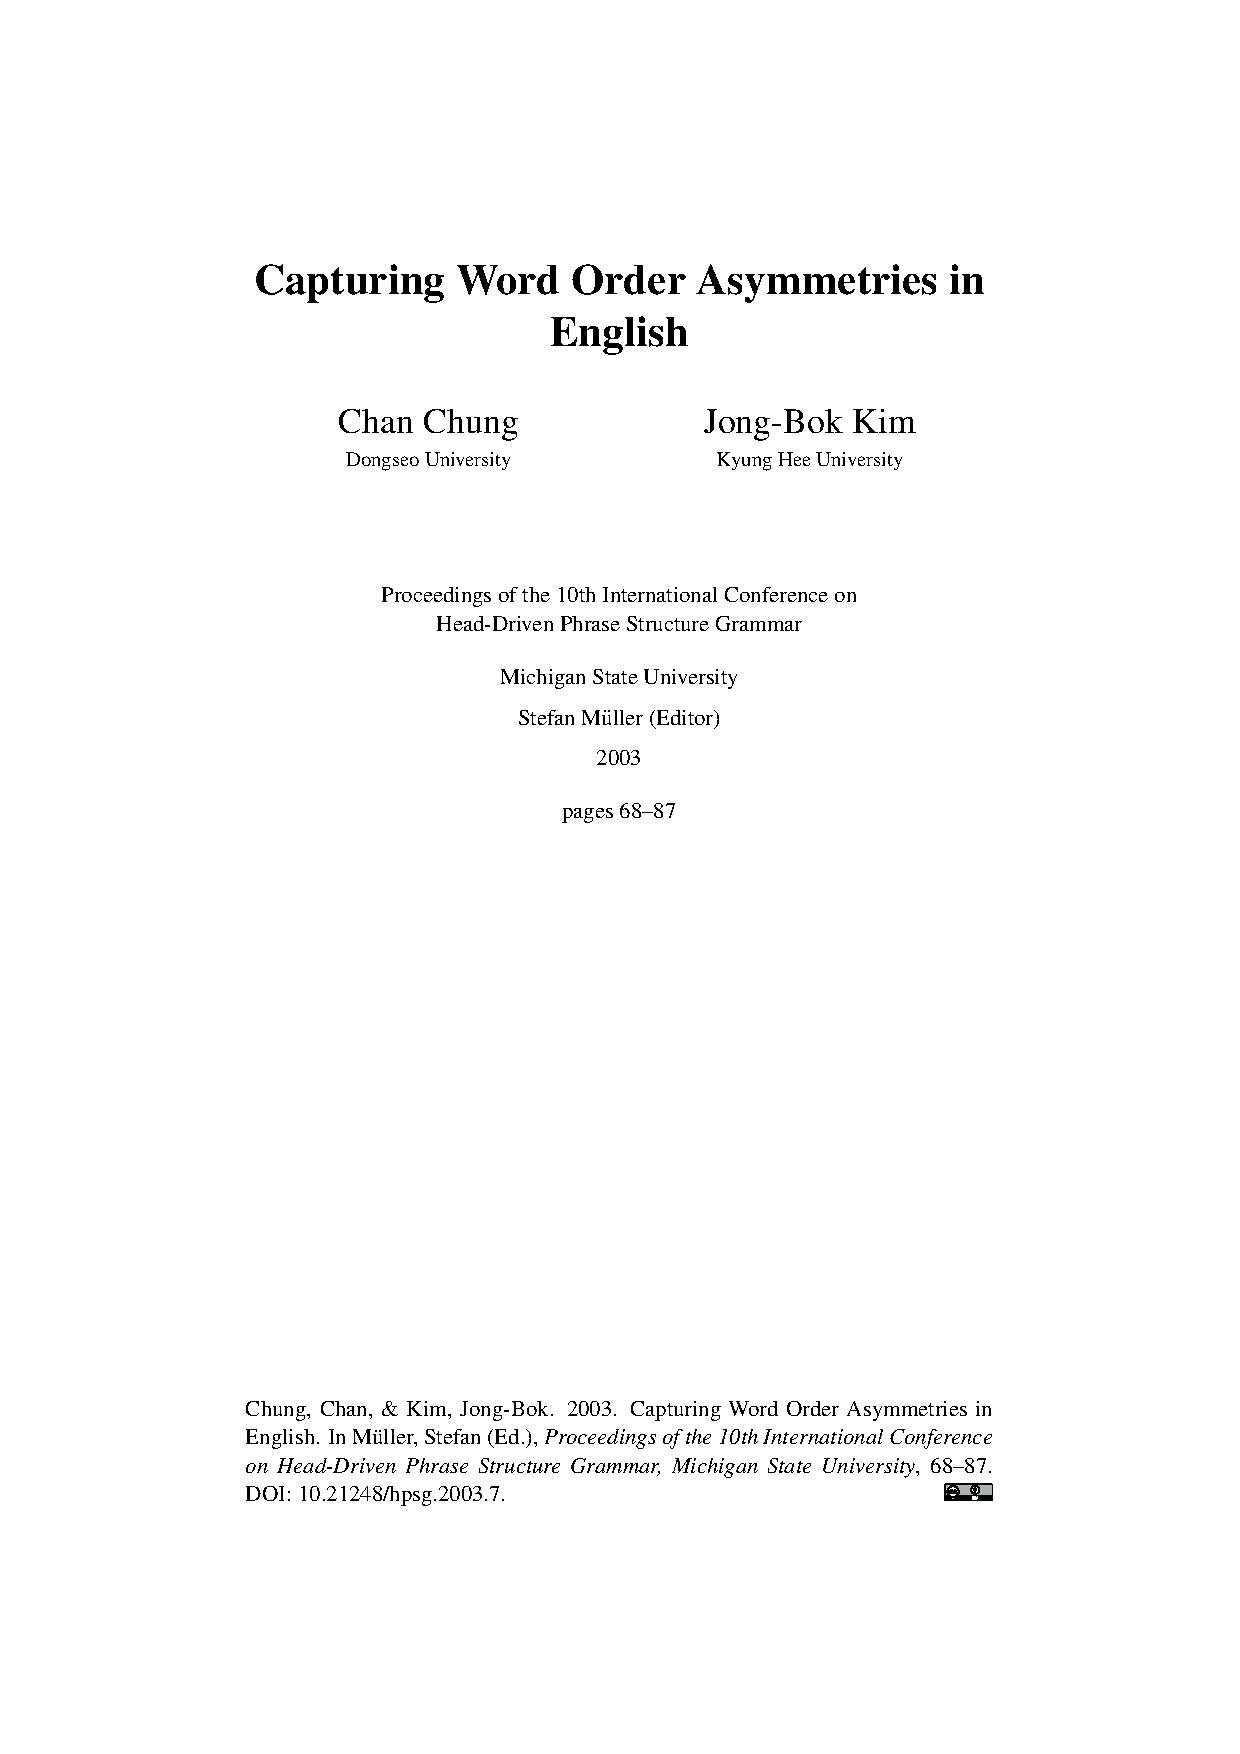
\includepdf[pages=-,pagecommand=\thispagestyle{plain},
            addtotoc={1,section,1,
            {Chan Chung and Jong-Bok Kim: Capturing Word Order Asymmetries in English Left-Peripheral Constructions: A Domain-Based Approach},
             ck}]{chung-kim.pdf}

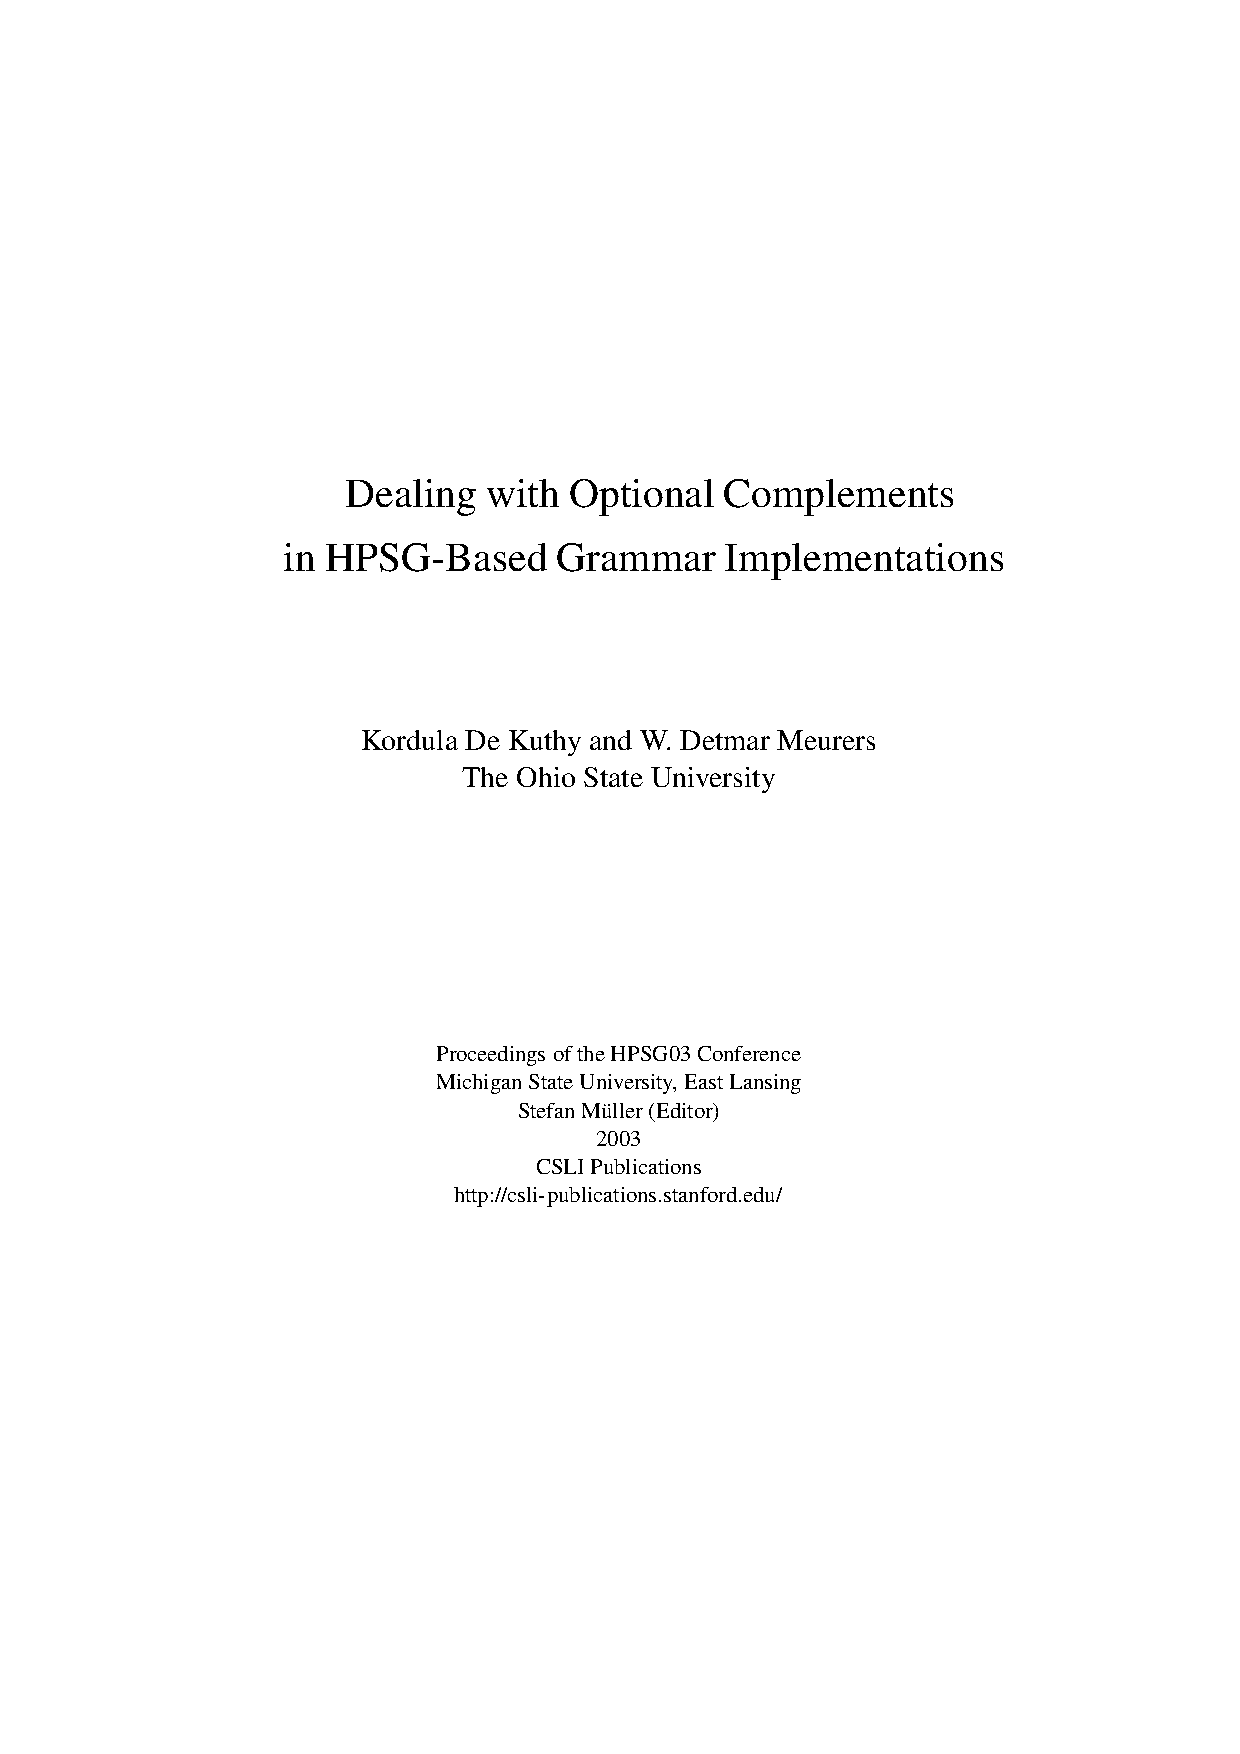
\includepdf[pages=-,pagecommand=\thispagestyle{plain},
            addtotoc={1,section,1,
            {Kordula De Kuthy and W. Detmar Meurers: Dealing with Optional Complements in HPSG-Based Grammar Implementations},
             dkm-o}]{dekuthy-meurers-optionality.pdf}

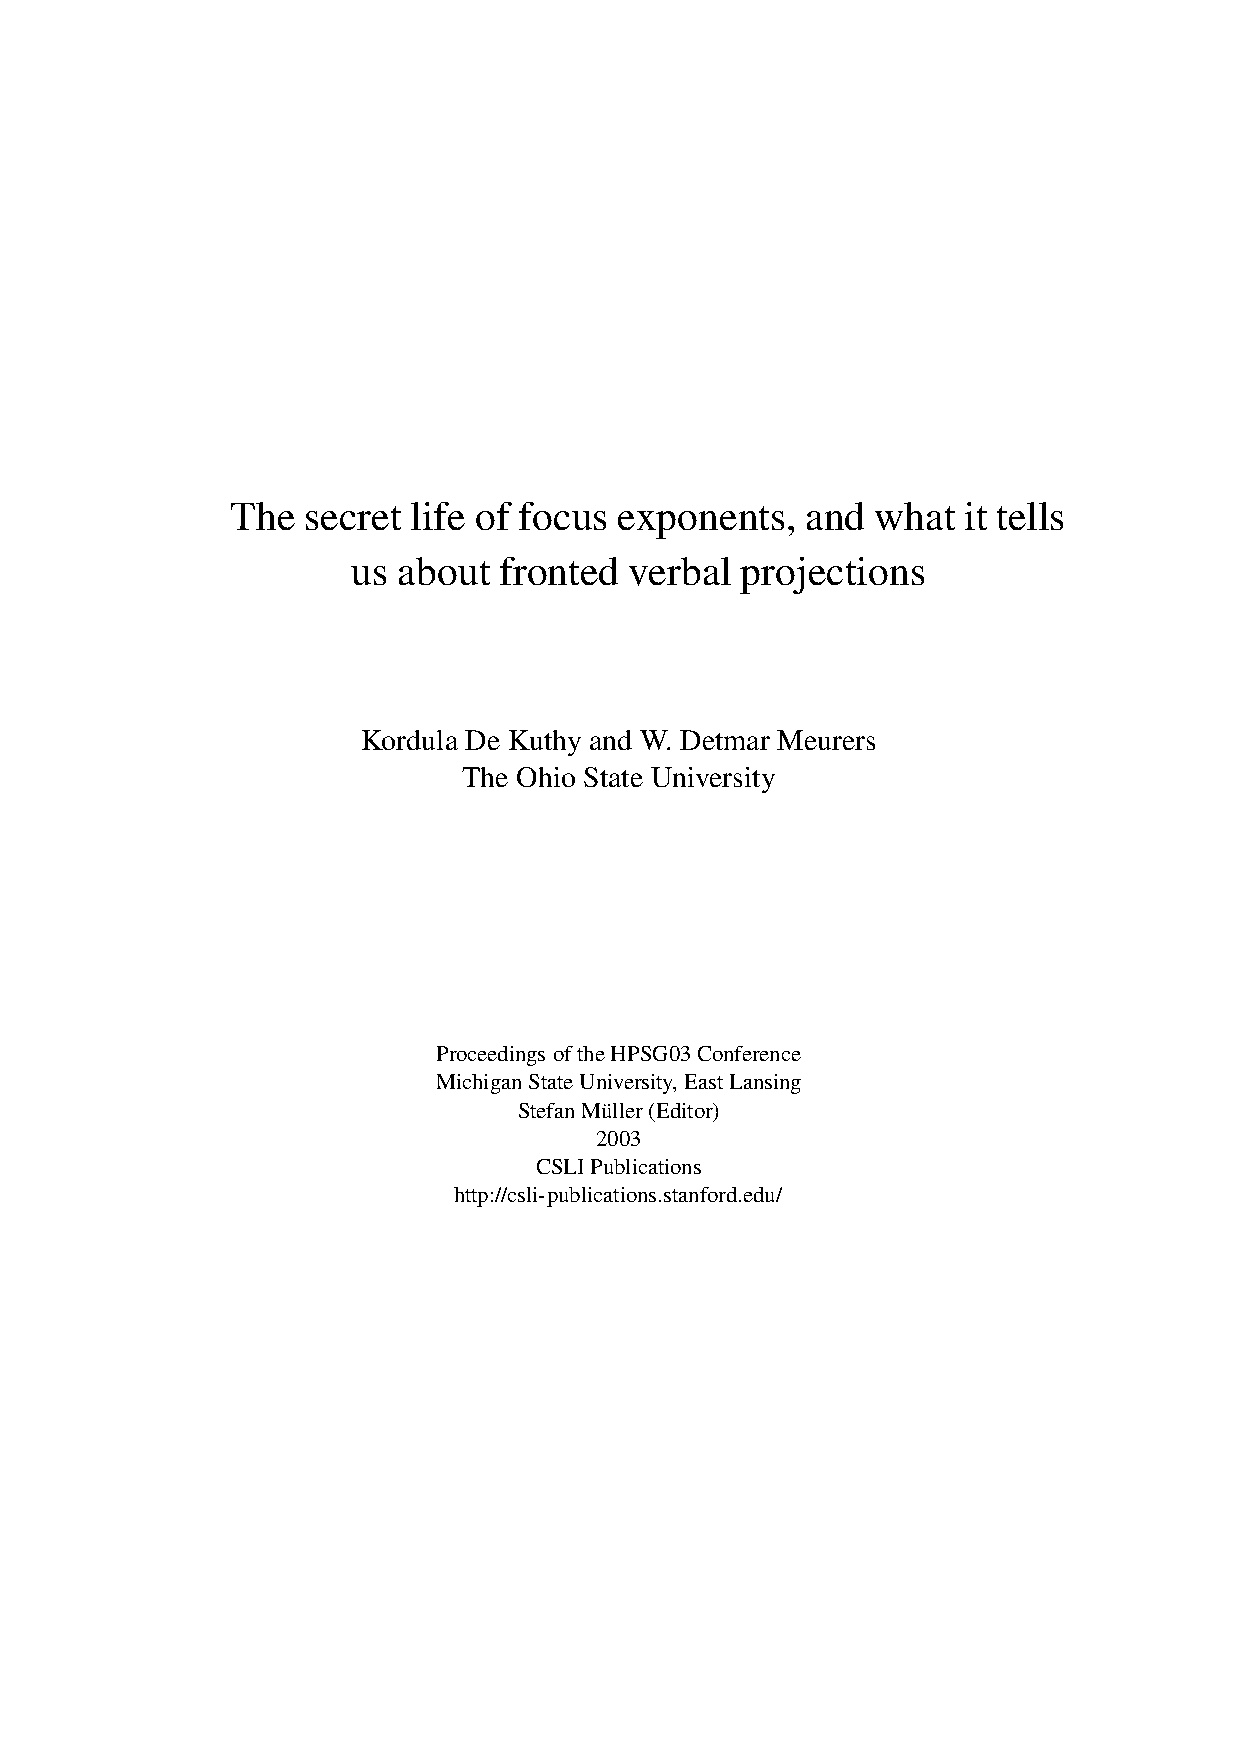
\includepdf[pages=-,pagecommand=\thispagestyle{plain},
            addtotoc={1,section,1,
            {Kordula De Kuthy and W. Detmar Meurers: The Secret Life of Focus Exponents, and What it Tells Us about Fronted Verbal Projections},
             dkm-f}]{dekuthy-meurers-focus.pdf}


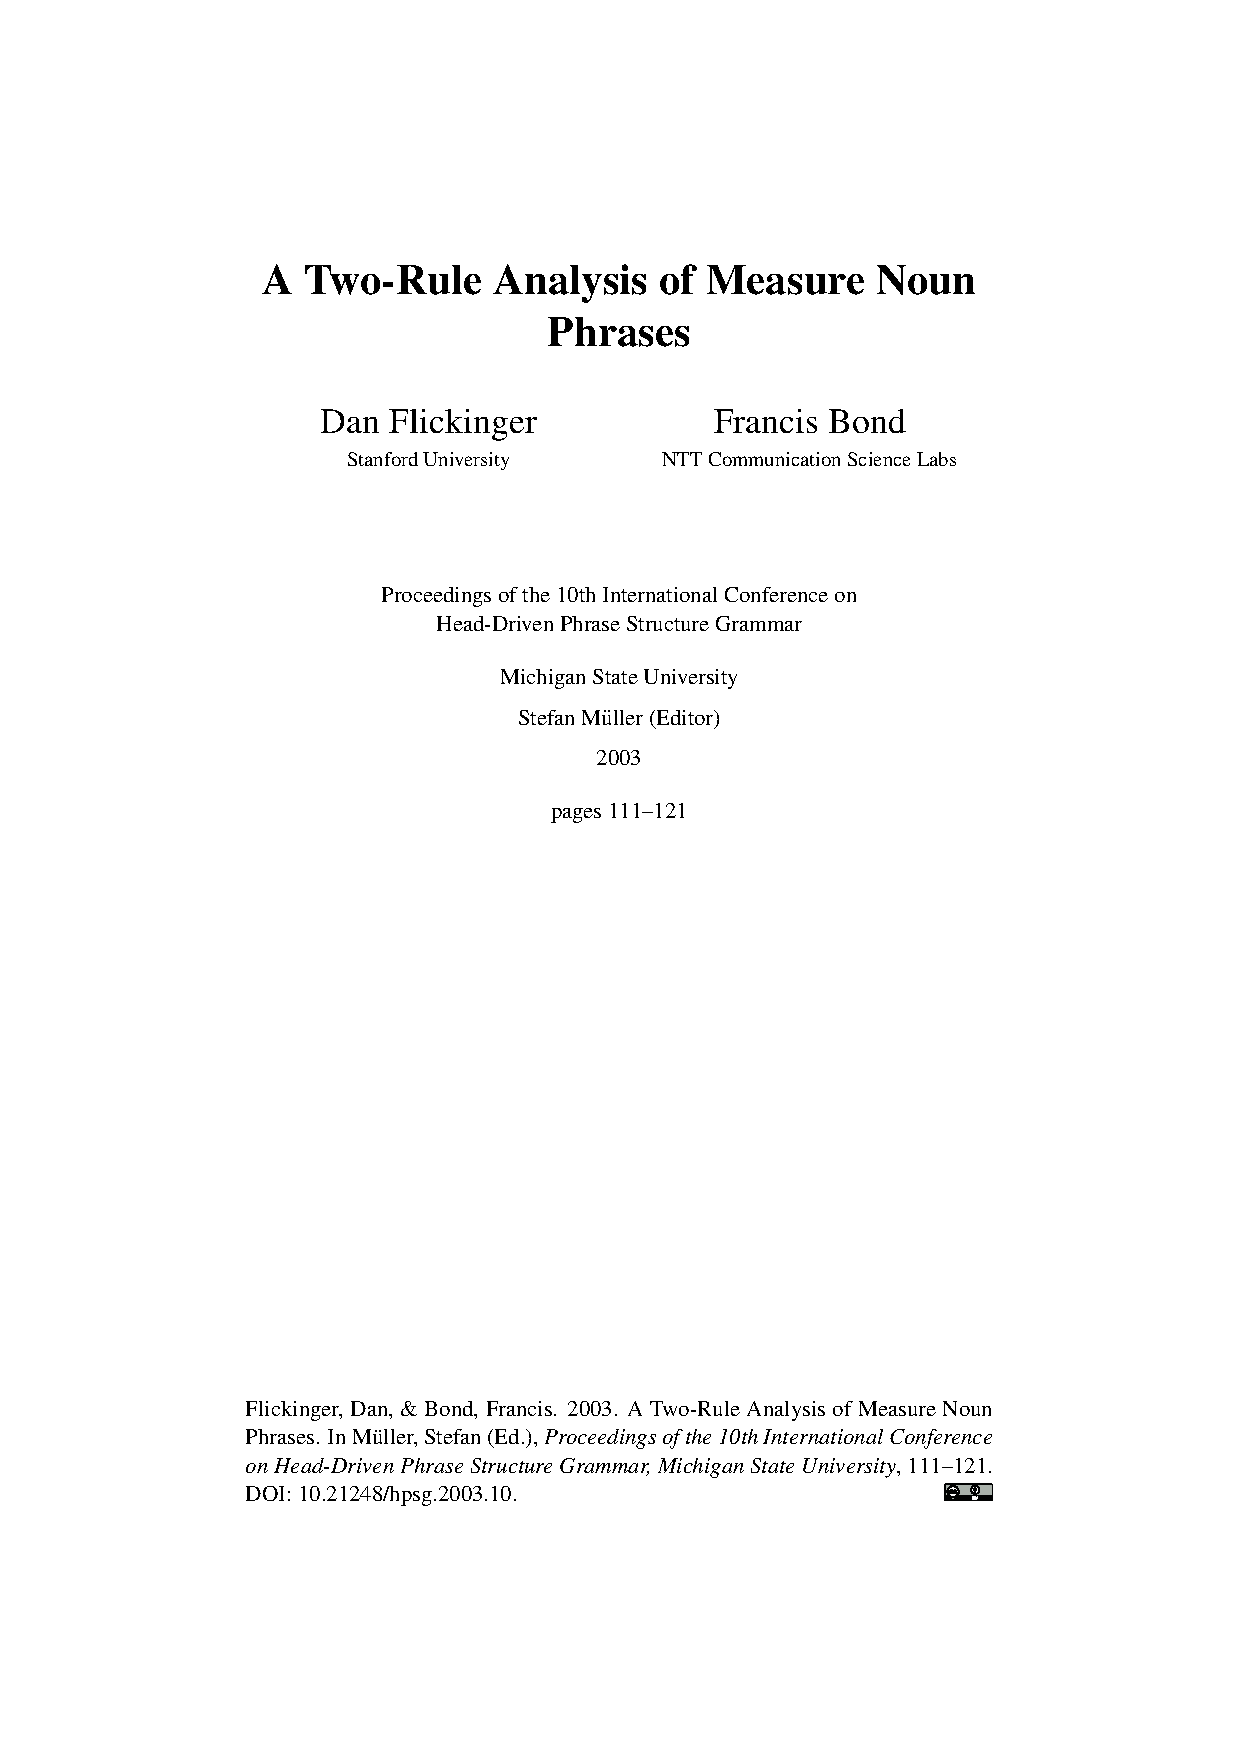
\includepdf[pages=-,pagecommand=\thispagestyle{plain},
            addtotoc={1,section,1,
            {Dan Flickinger and Francis Bond: A Two-Rule Analysis of Measure Noun Phrases},
             fb}]{flickinger-bond.pdf}

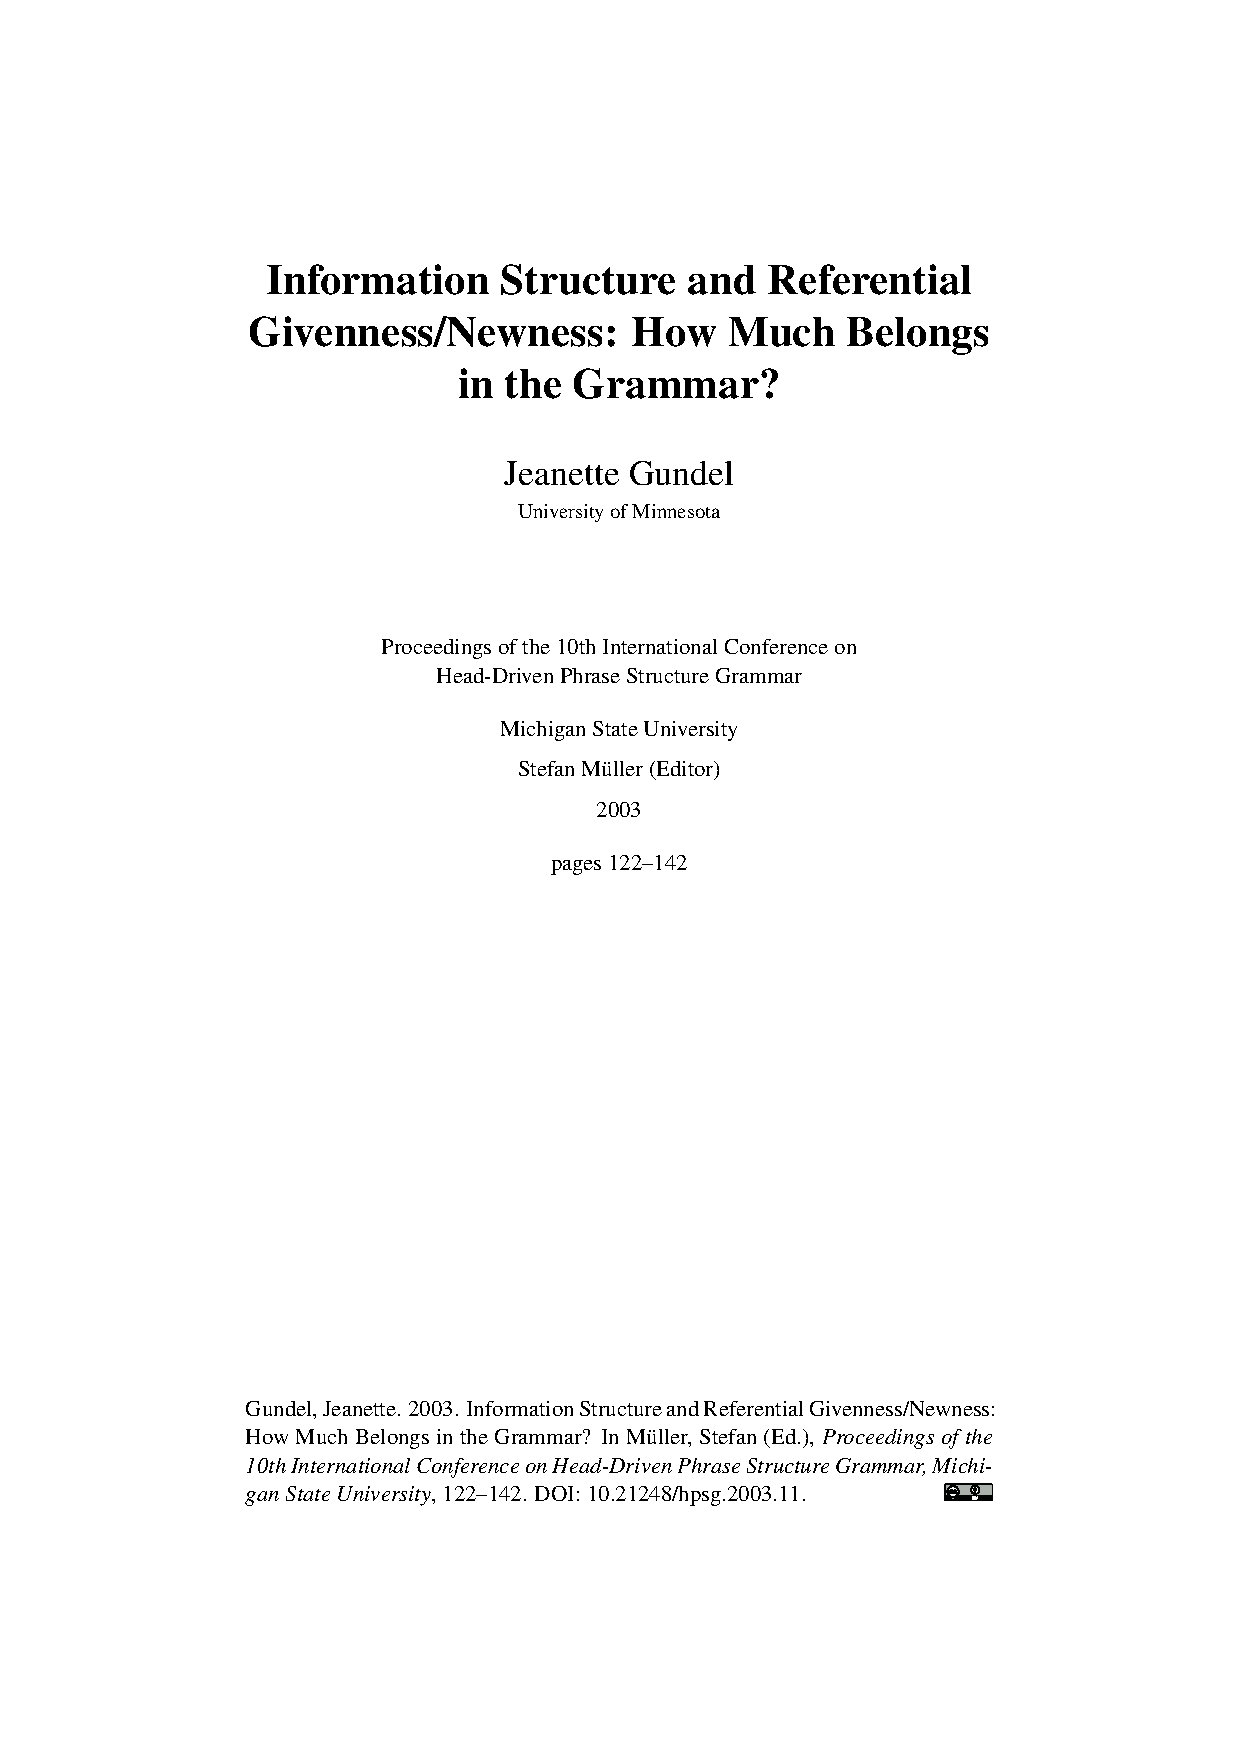
\includepdf[pages=-,pagecommand=\thispagestyle{plain},
            addtotoc={1,section,1,
            {Jeanette Gundel: Information Structure and Referential Givenness/Newness: How Much Belongs in the Grammar?},
             gundel}]{gundel.pdf}

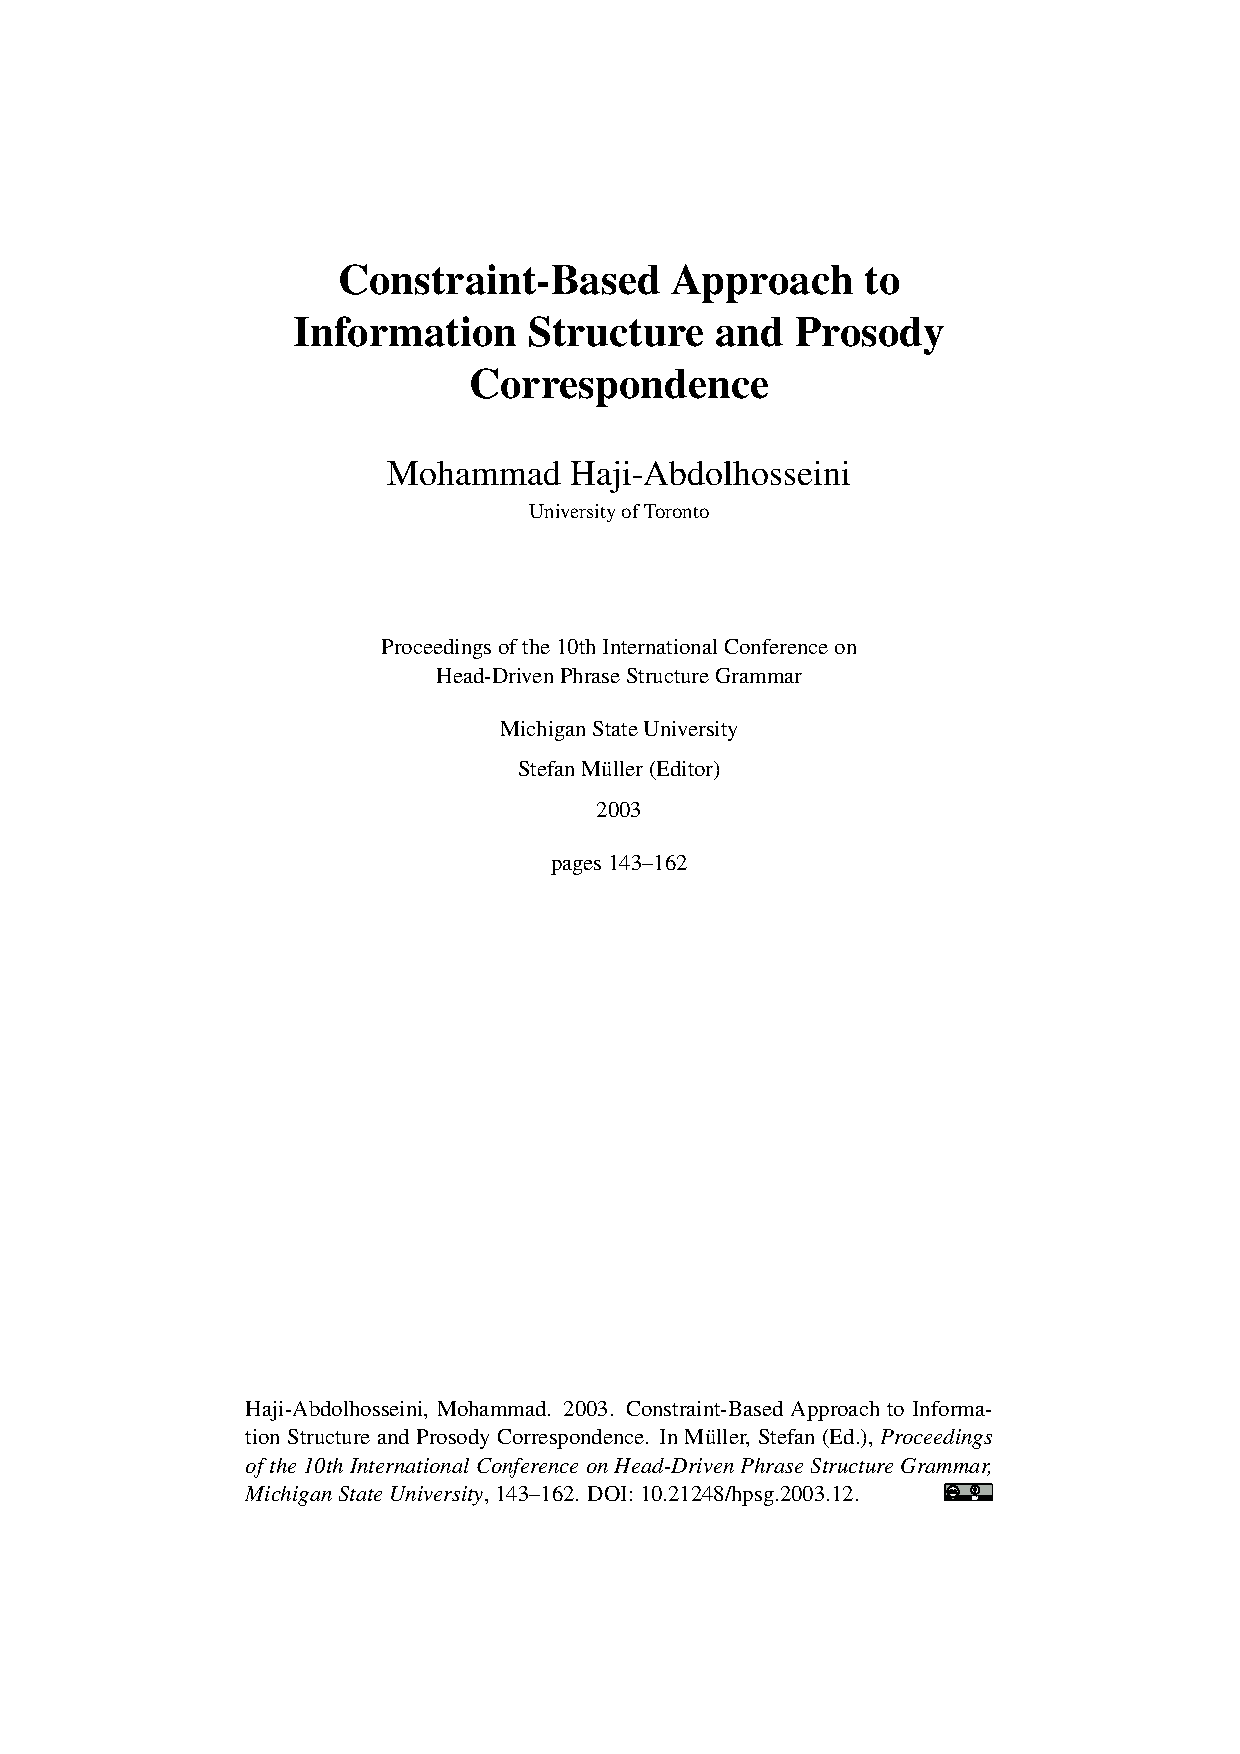
\includepdf[pages=-,pagecommand=\thispagestyle{plain},
            addtotoc={1,section,1,
           {Mohammad Haji-Abdolhosseini: A Constraint-Based Approach to Information Structure and Prosody Correspondence},
            haji}]{haji-abdolhosseini.pdf}

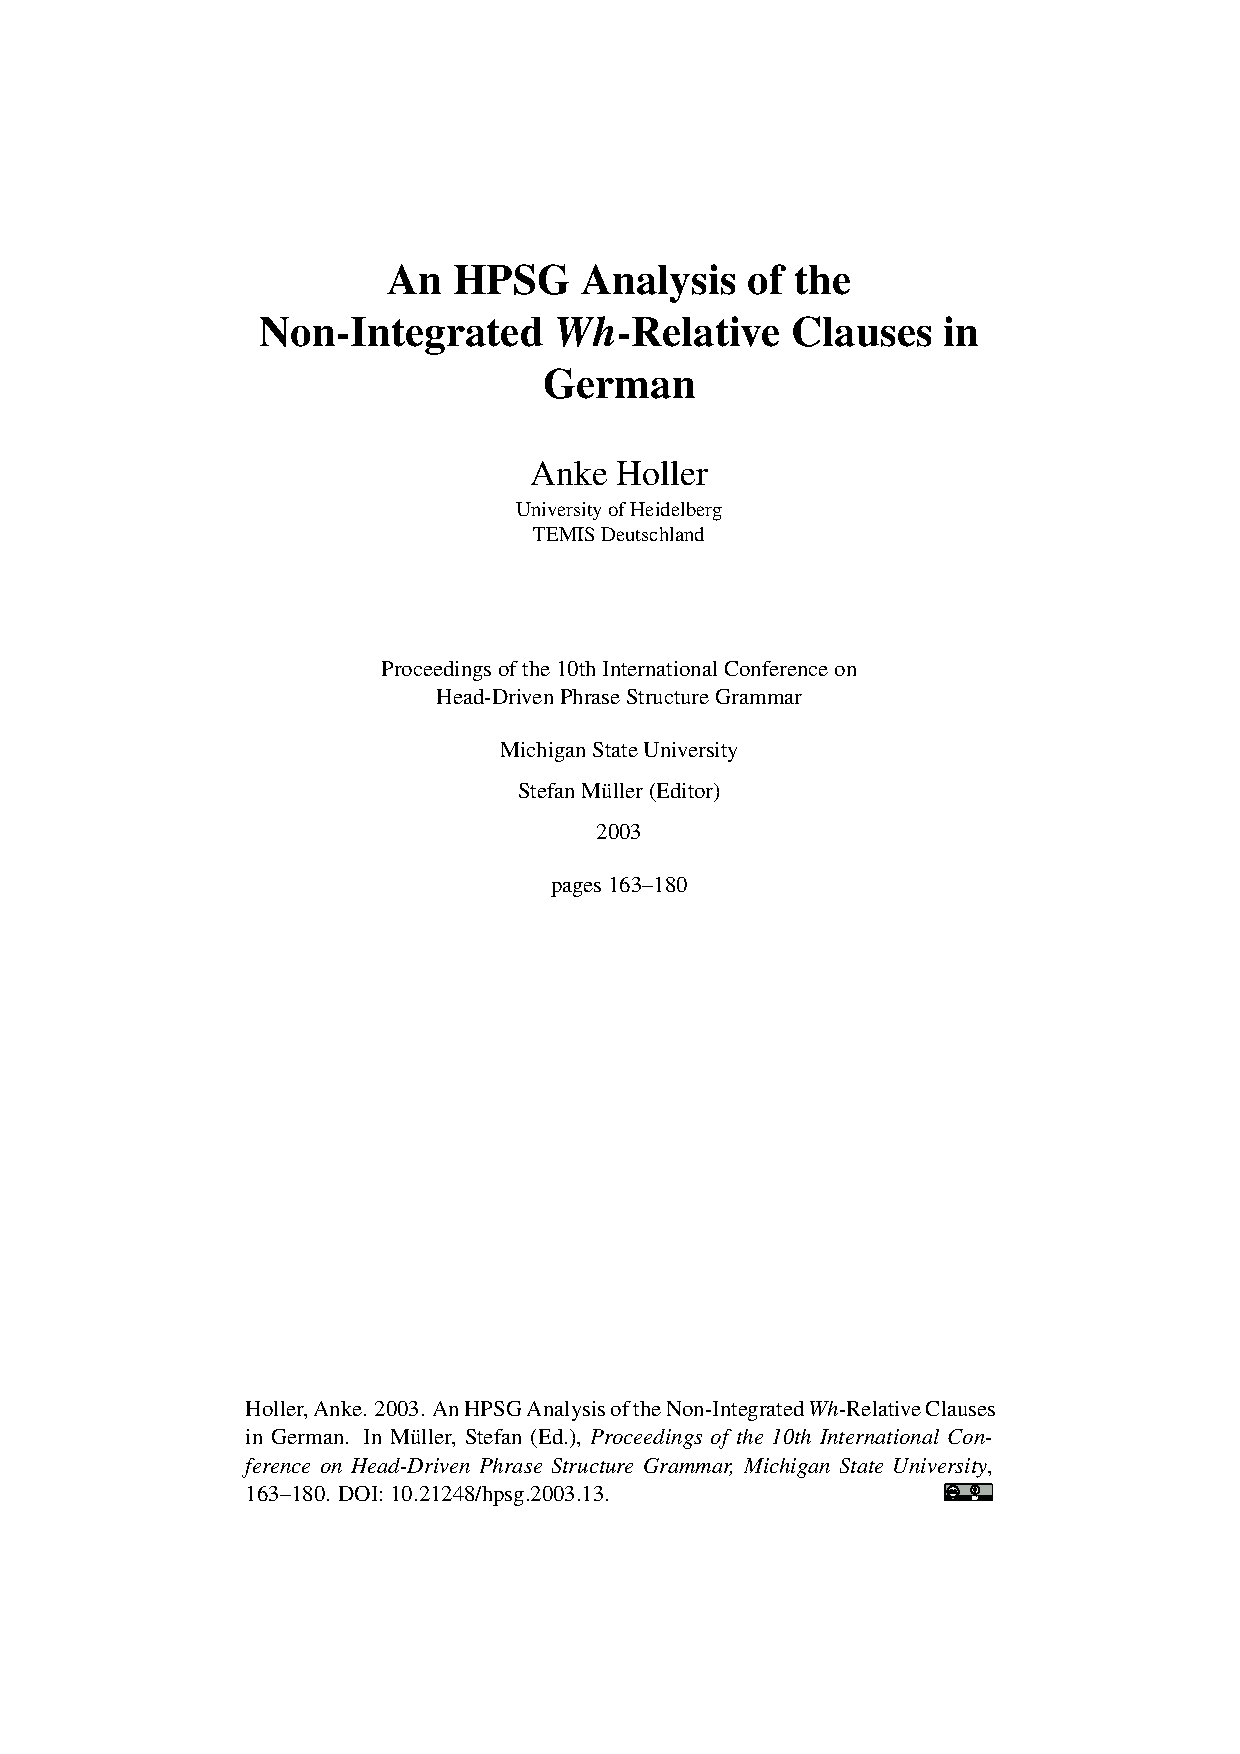
\includepdf[pages=-,pagecommand=\thispagestyle{plain},
            addtotoc={1,section,1,
           {Anke Holler: An HPSG Analysis of the Non-Integrated Wh-Relative Clauses in German},
            holler}]{holler.pdf}

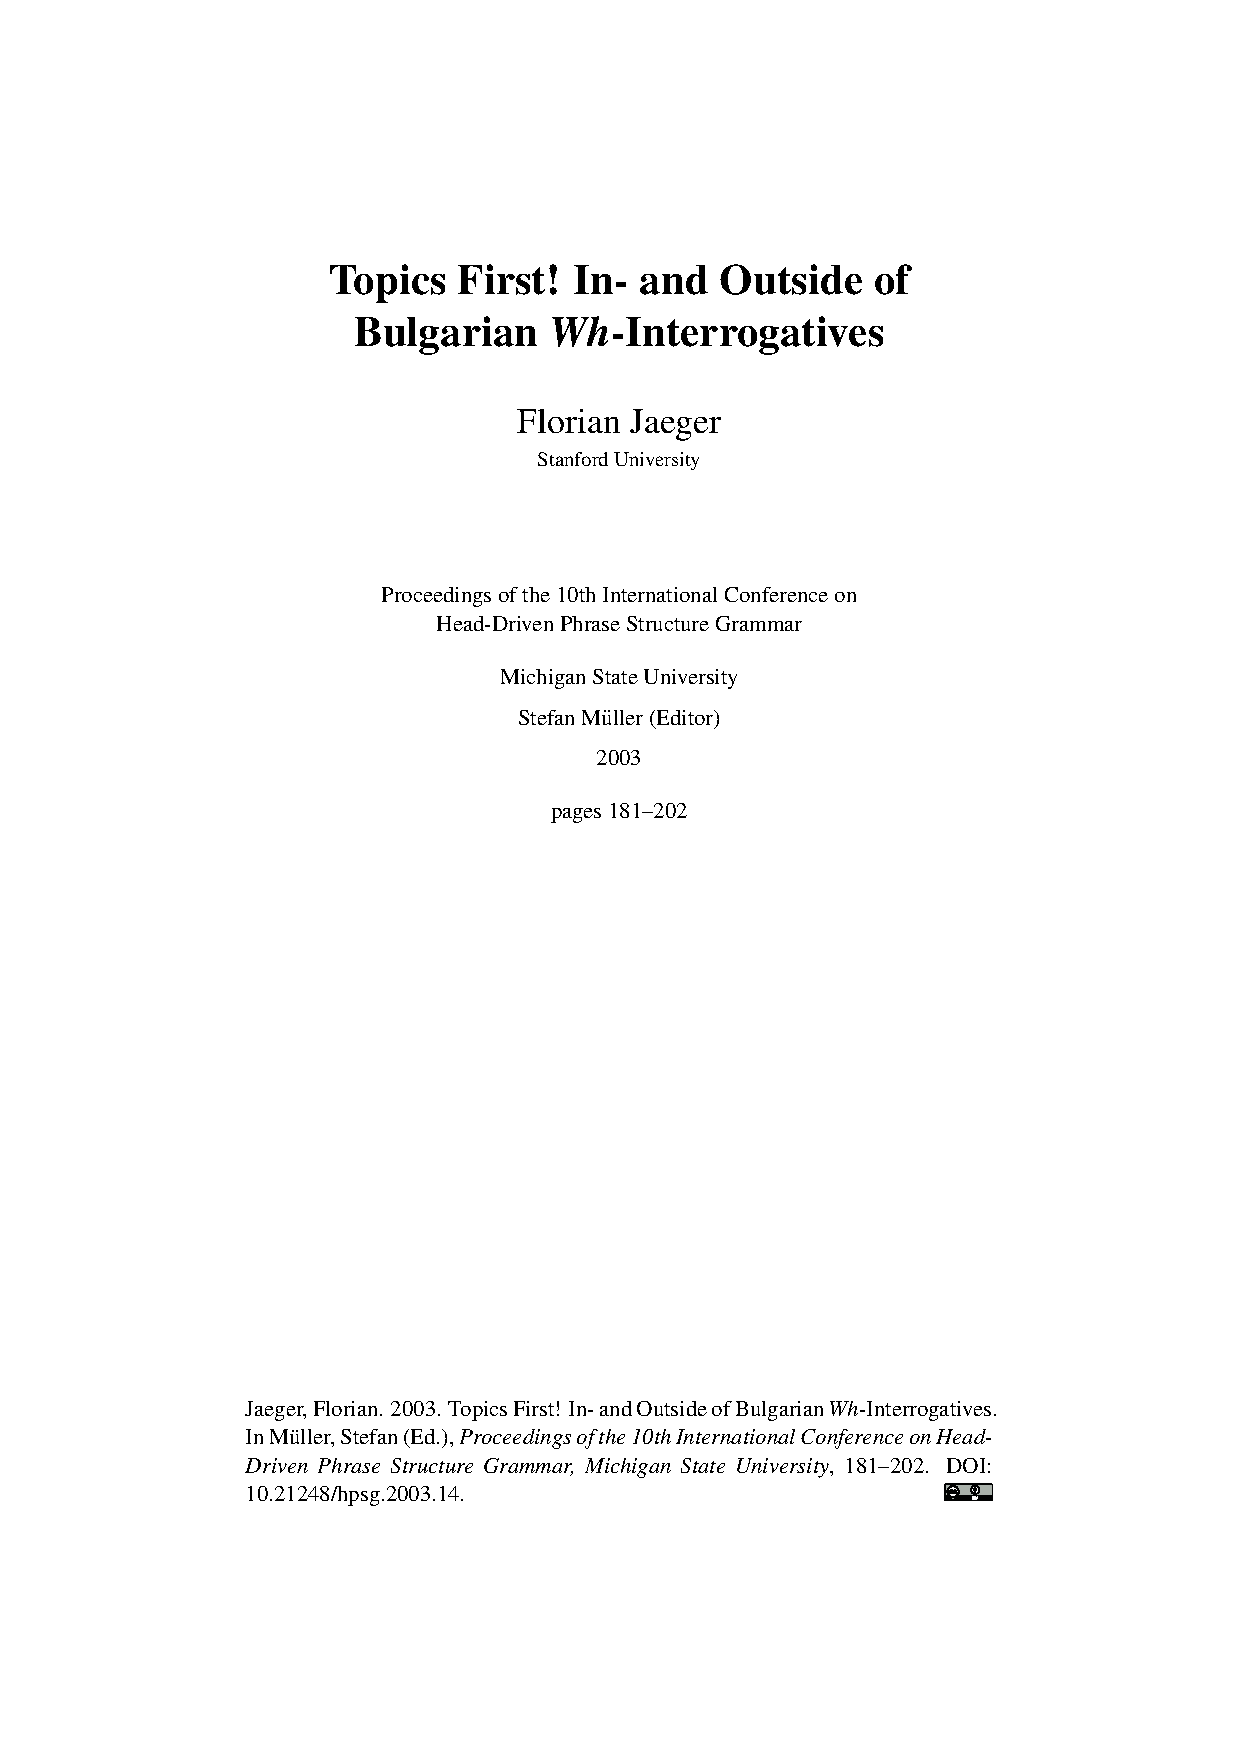
\includepdf[pages=-,pagecommand=\thispagestyle{plain},
            addtotoc={1,section,1,
           {Florian Jaeger: Topics First! In- and Outside of Bulgarian Wh-Interrogatives},
            jaeger}]{jaeger.pdf}

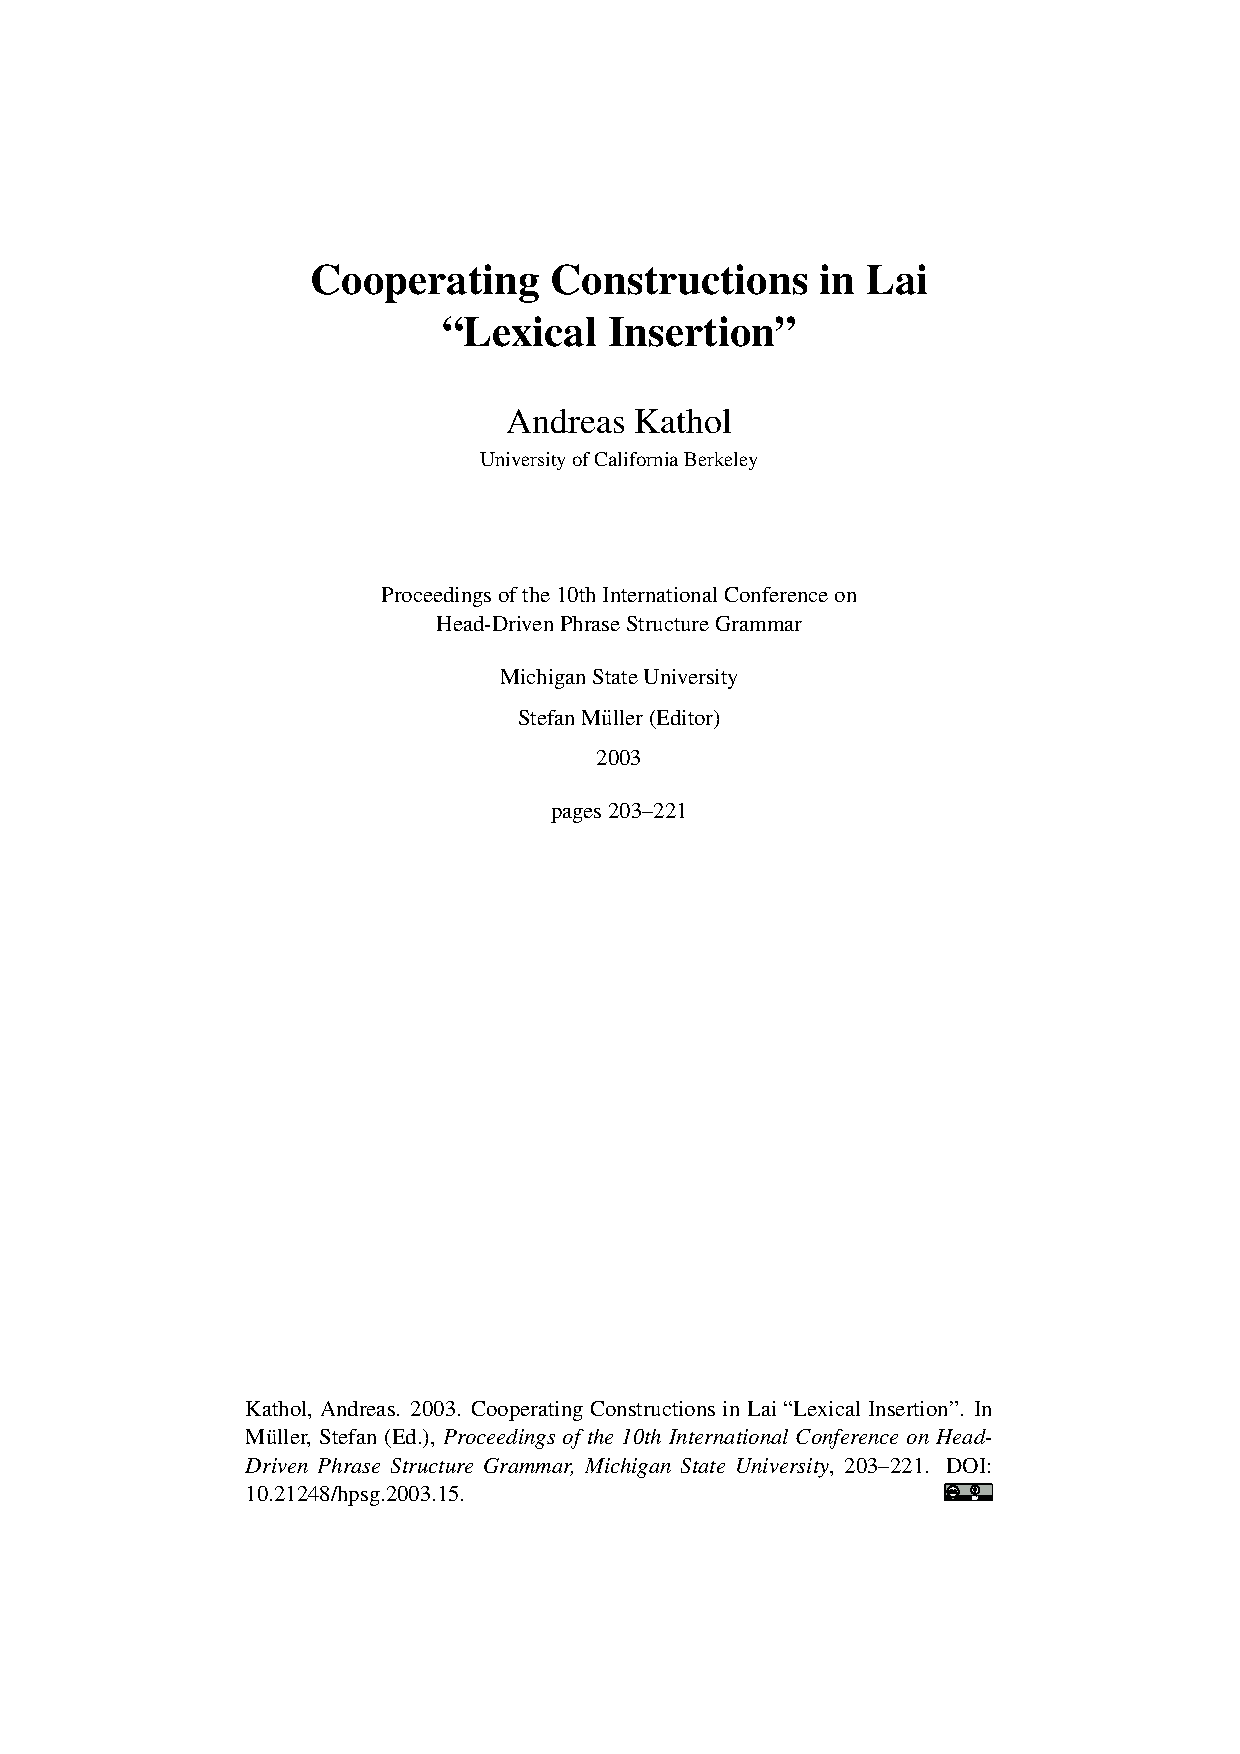
\includepdf[pages=-,pagecommand=\thispagestyle{plain},
            addtotoc={1,section,1,
           {Andreas Kathol: Cooperating Constructions in Lai ``Lexical Insertion''},
            kathol}]{kathol.pdf}

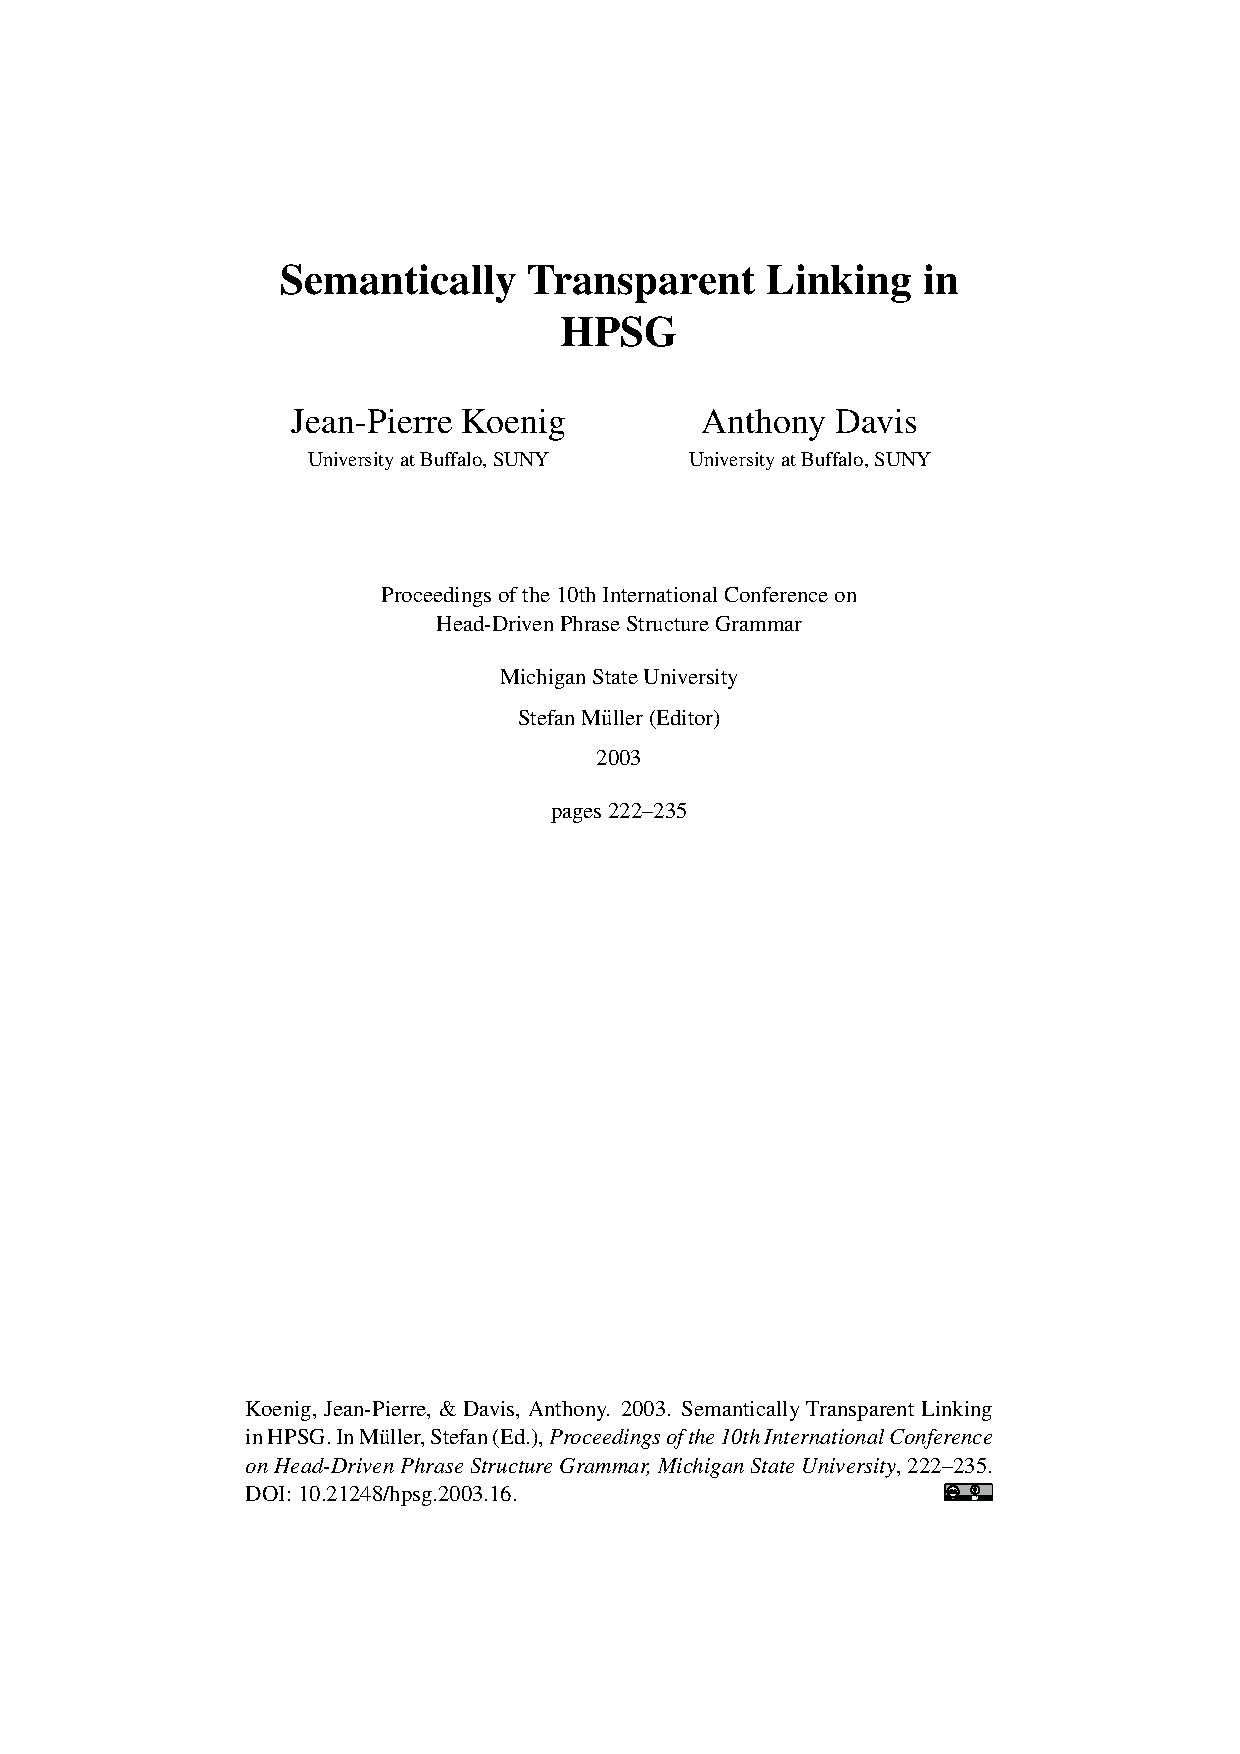
\includepdf[pages=-,pagecommand=\thispagestyle{plain},
            addtotoc={1,section,1,
            {Jean-Pierre Koenig and Anthony Davis: Semantically Transparent Linking in HPSG},
             koenig-davis}]{koenig-davis.pdf}

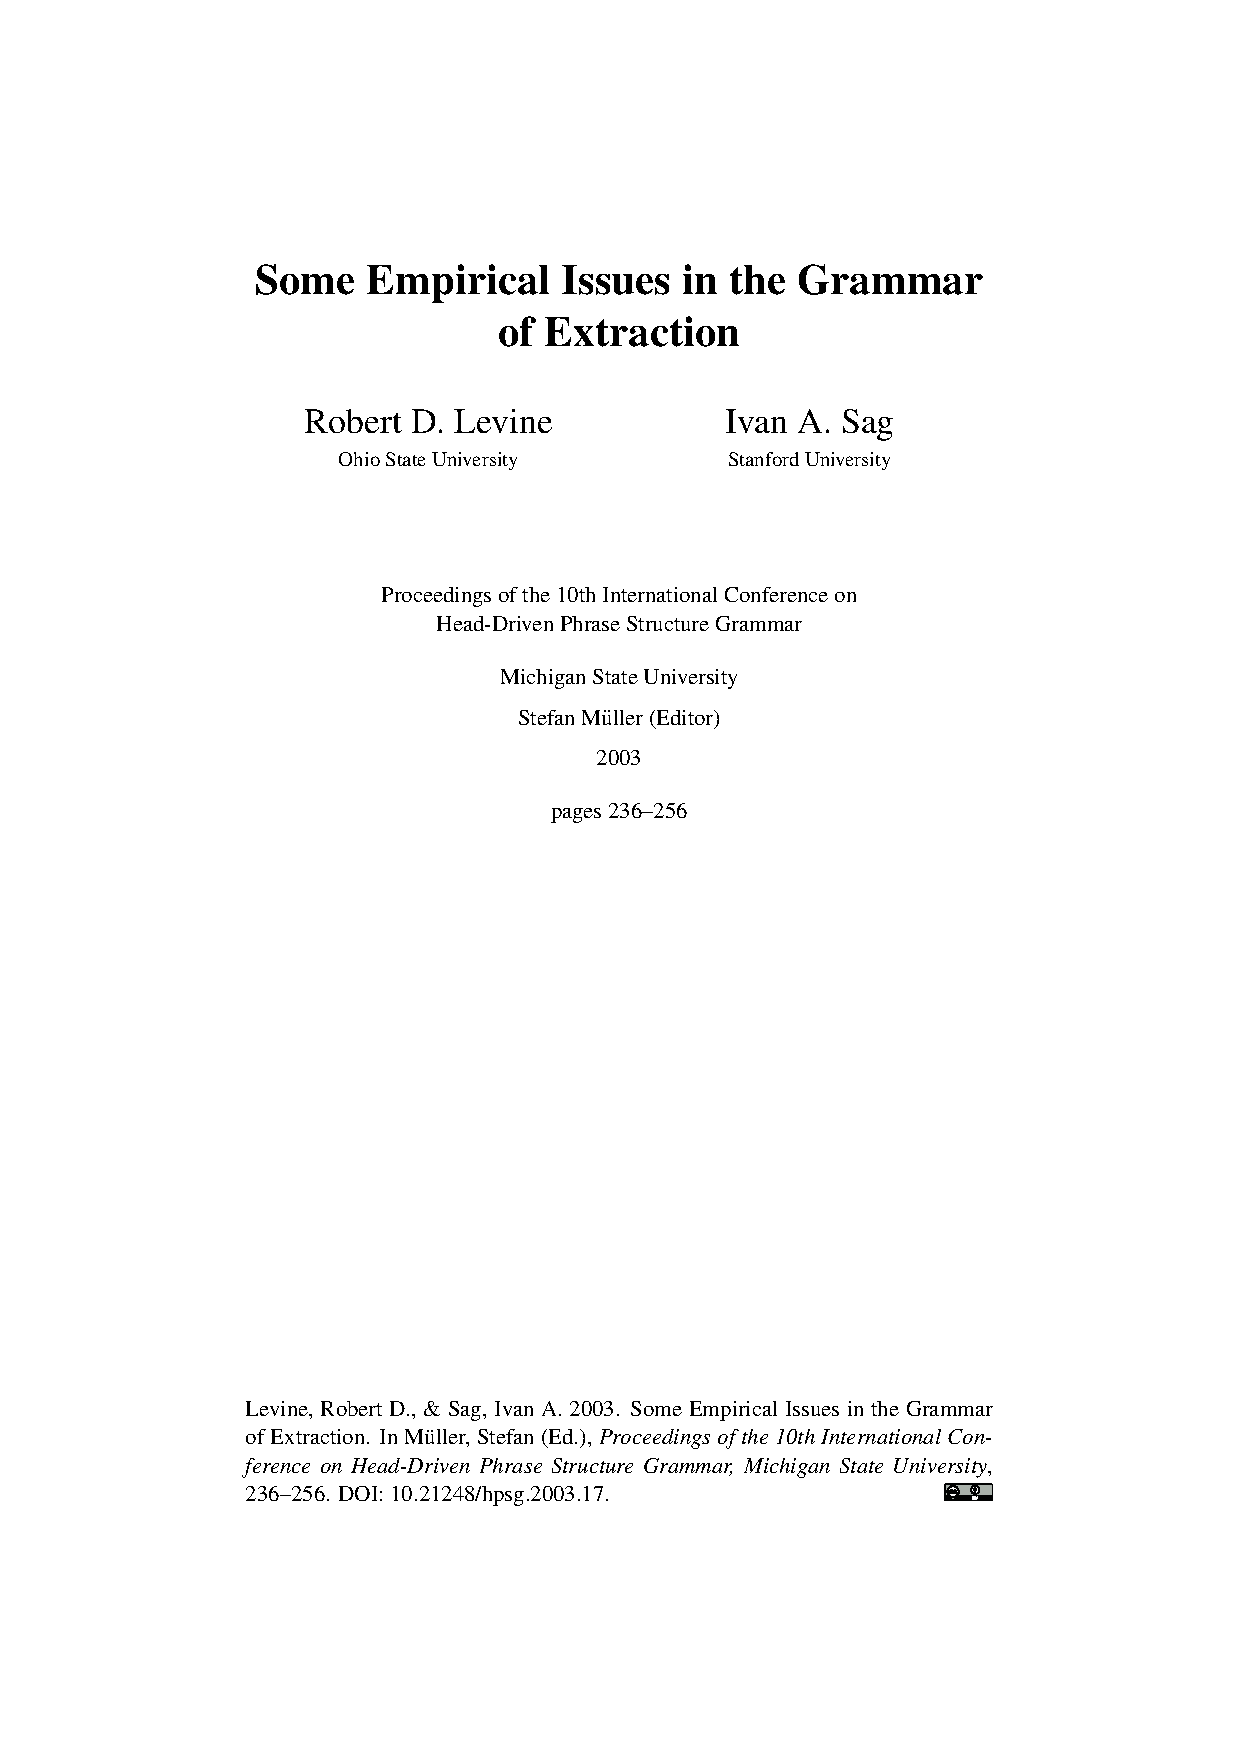
\includepdf[pages=-,pagecommand=\thispagestyle{plain},
            addtotoc={1,section,1,
            {Robert D. Levine and Ivan A. Sag: Some Empirical Issues in the Grammar of Extraction},
             levine-sag}]{levine-sag.pdf}


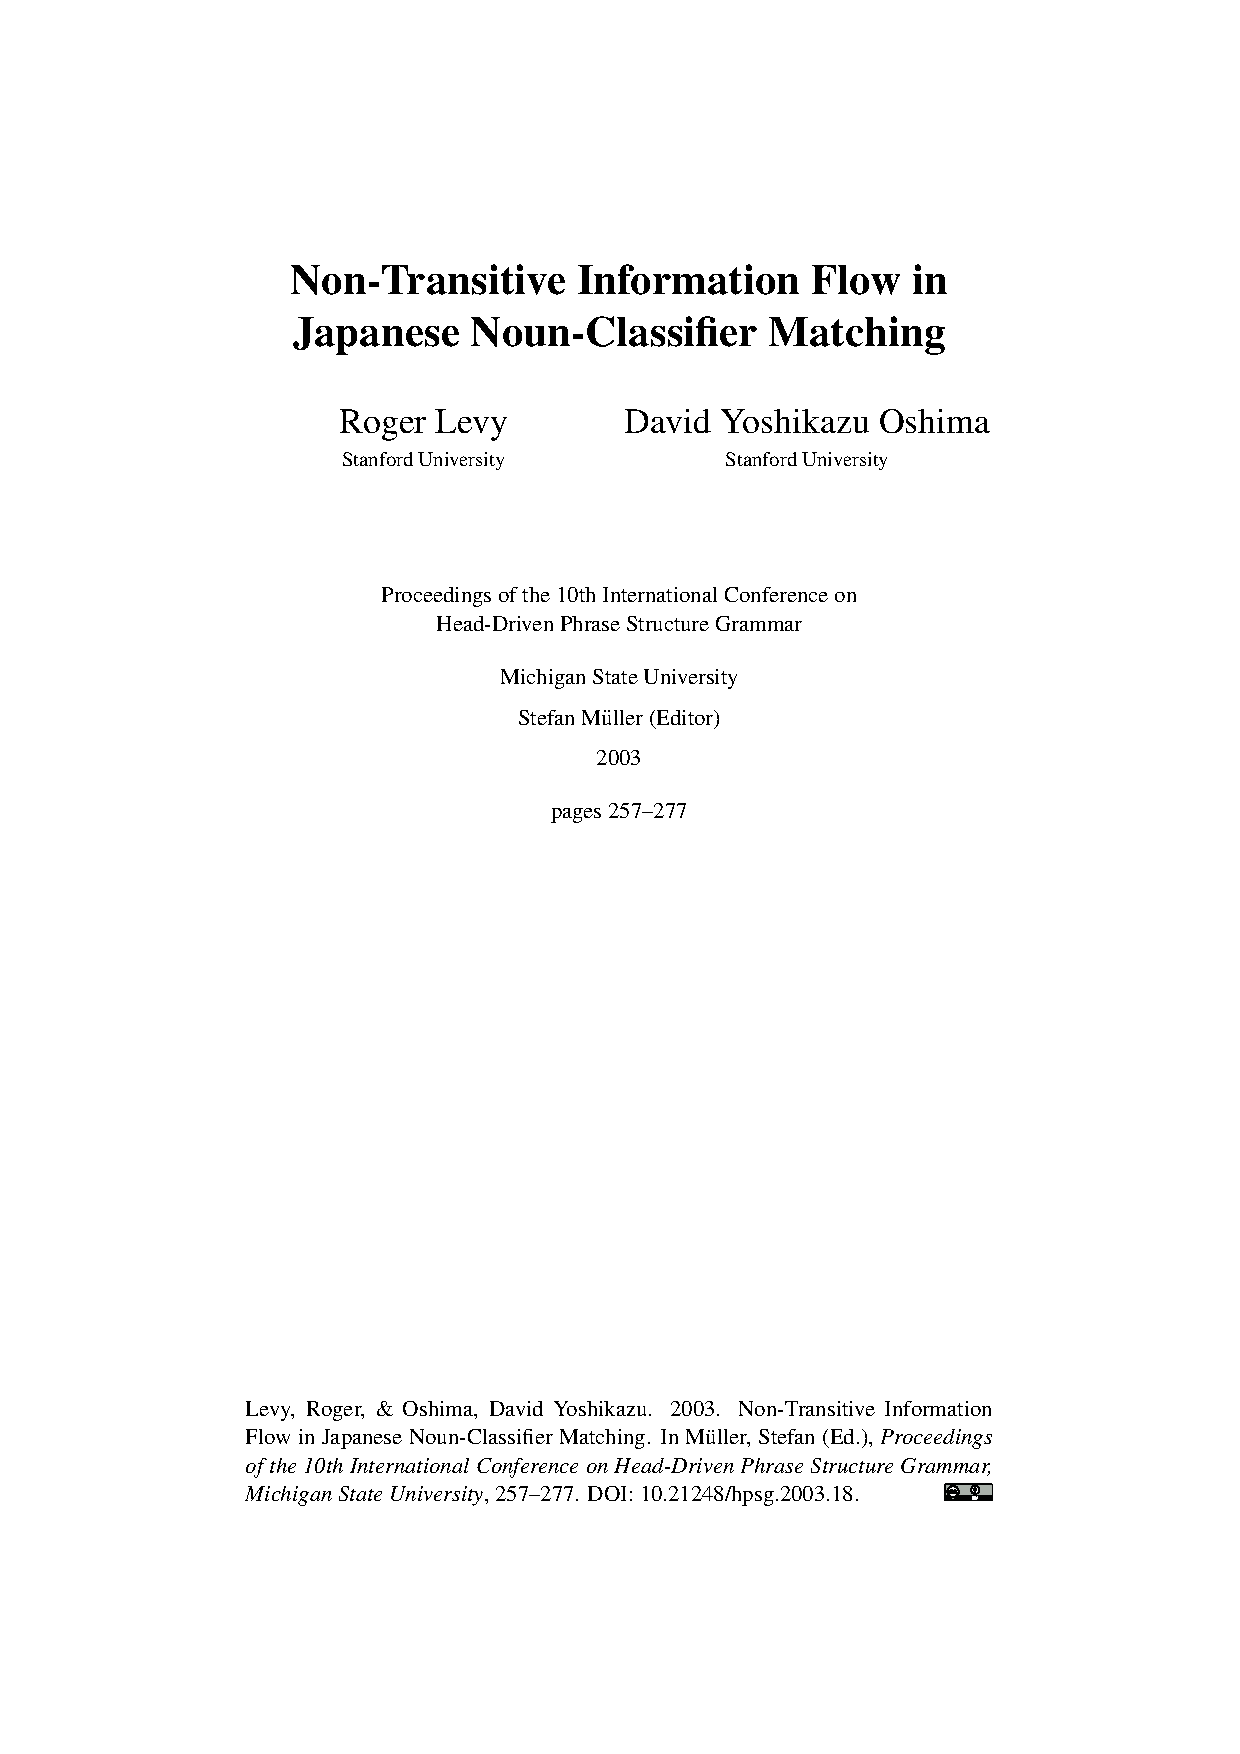
\includepdf[pages=-,pagecommand=\thispagestyle{plain},
            addtotoc={1,section,1,
            {Roger Levy and David Yoshikazu Oshima: Non-Transitive Information Flow in Japanese Noun-Classifier Matching},
             levy-oshima}]{levy-oshima.pdf}

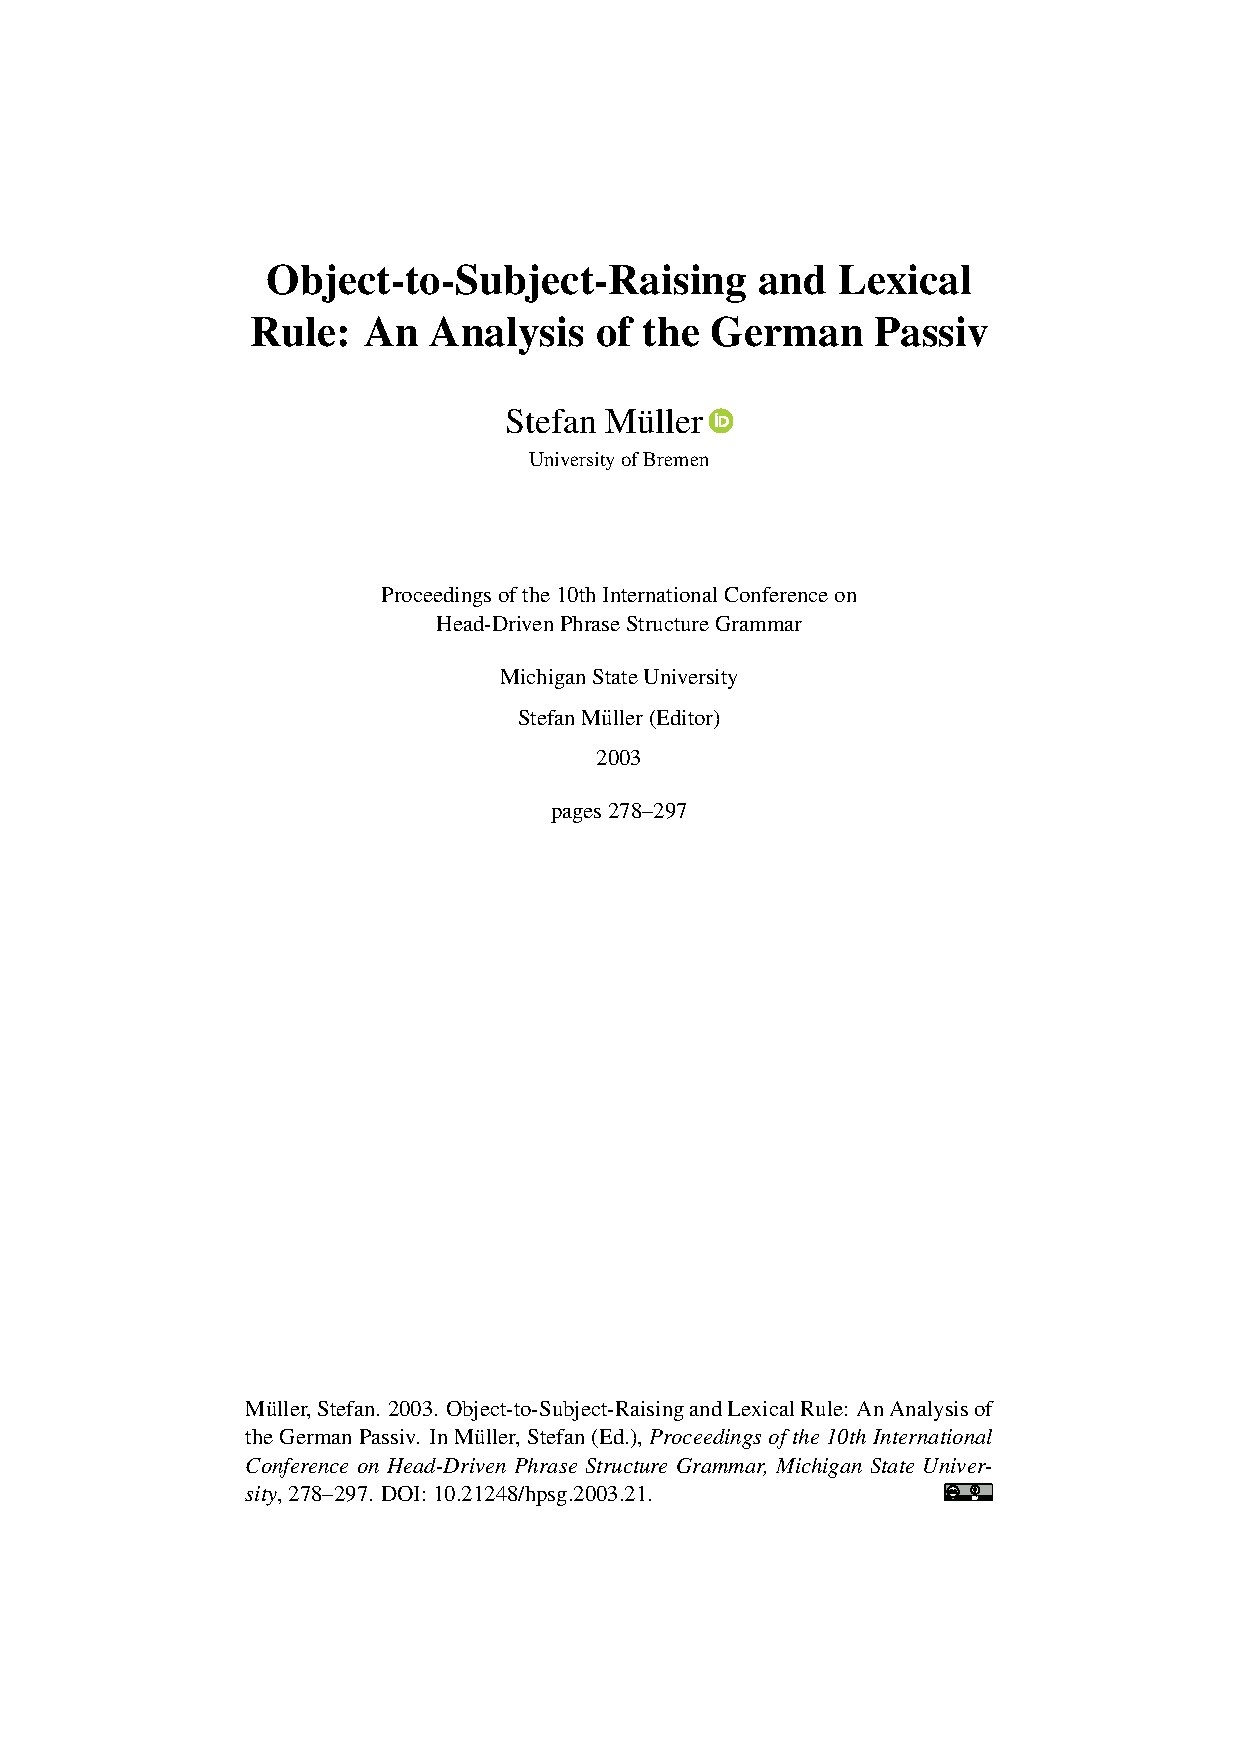
\includepdf[pages=-,pagecommand=\thispagestyle{plain},
            addtotoc={1,section,1,
            {Stefan M�ller: Object-to-Subject-Raising and Lexical Rule: An Analysis of the German Passive},
             mueller}]{mueller.pdf}


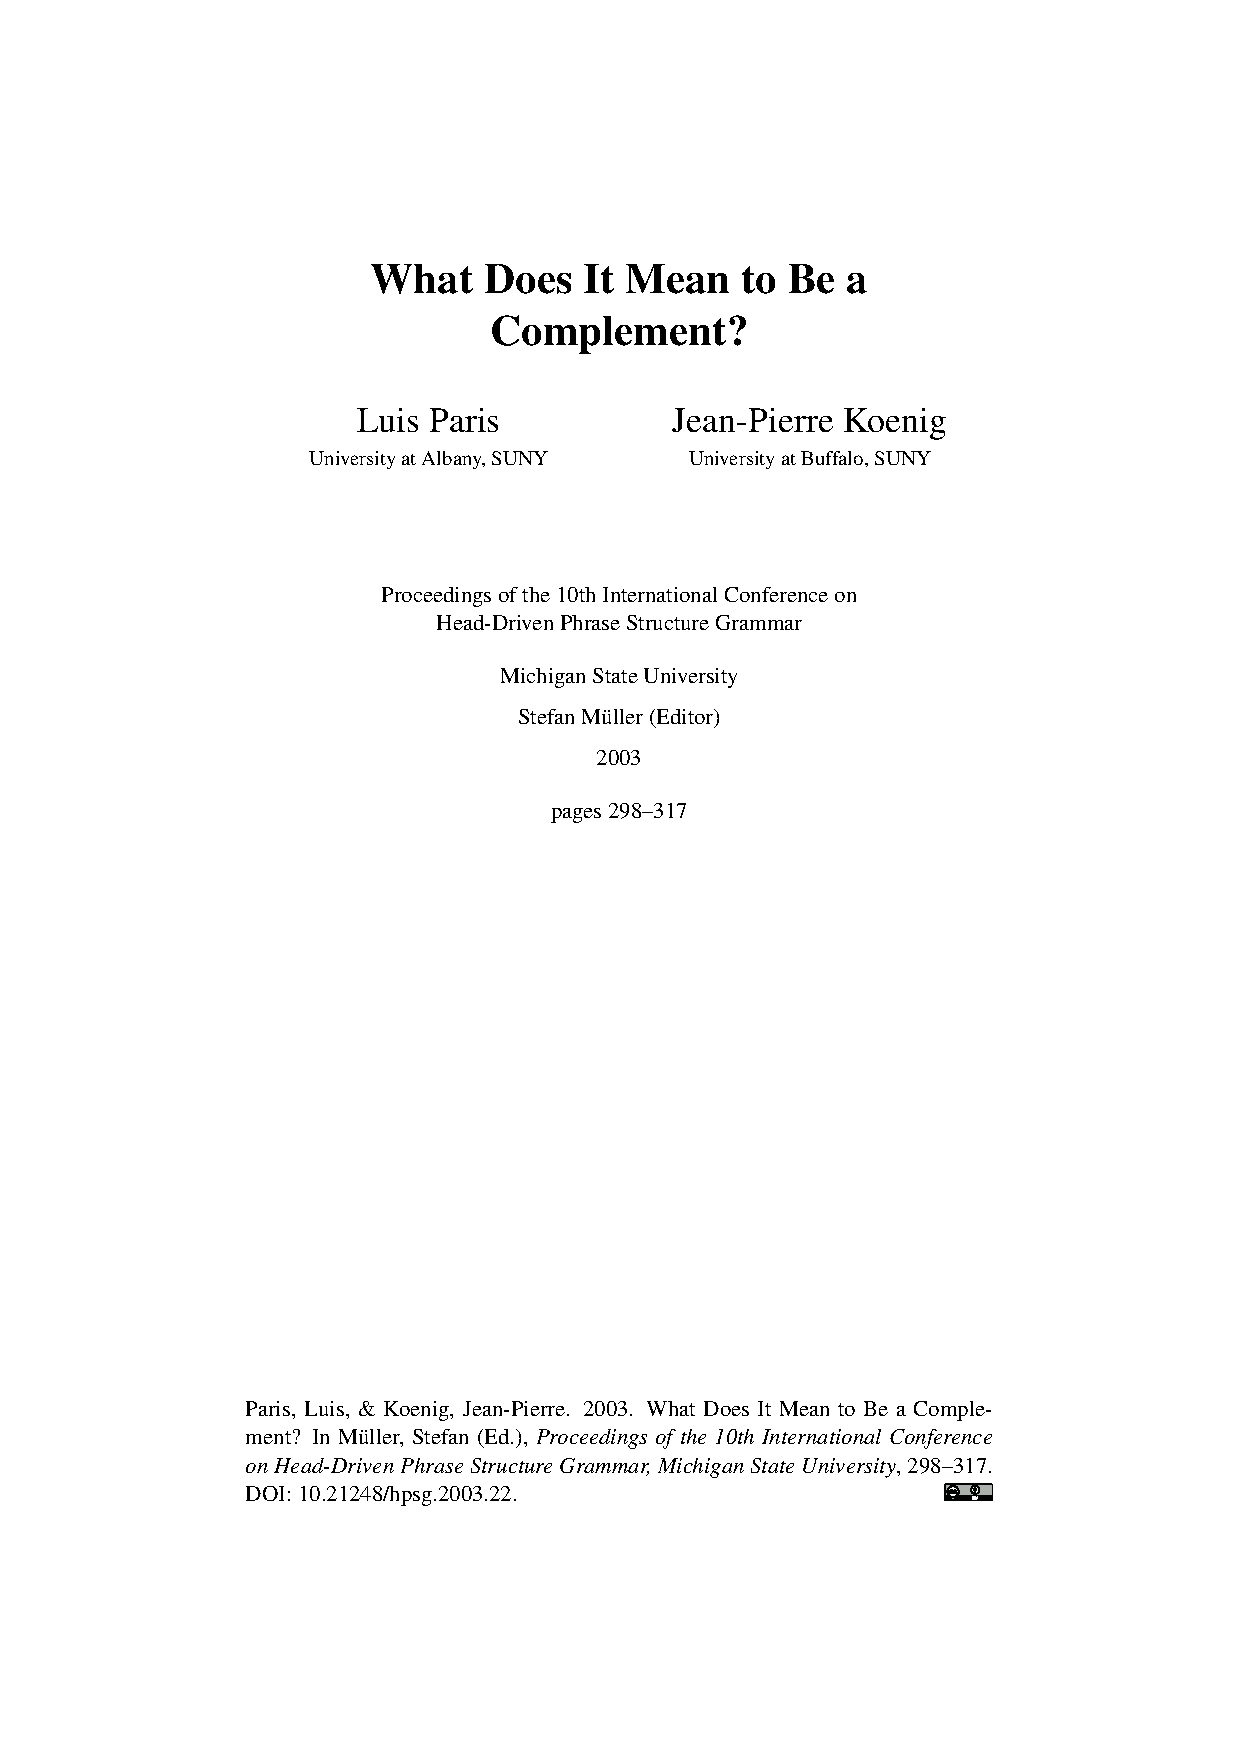
\includepdf[pages=-,pagecommand=\thispagestyle{plain},
            addtotoc={1,section,1,
            {Luis Paris and Jean-Pierre Koenig: What Does It Mean to Be a Complement?},
             paris-koeni}]{paris-koenig.pdf}

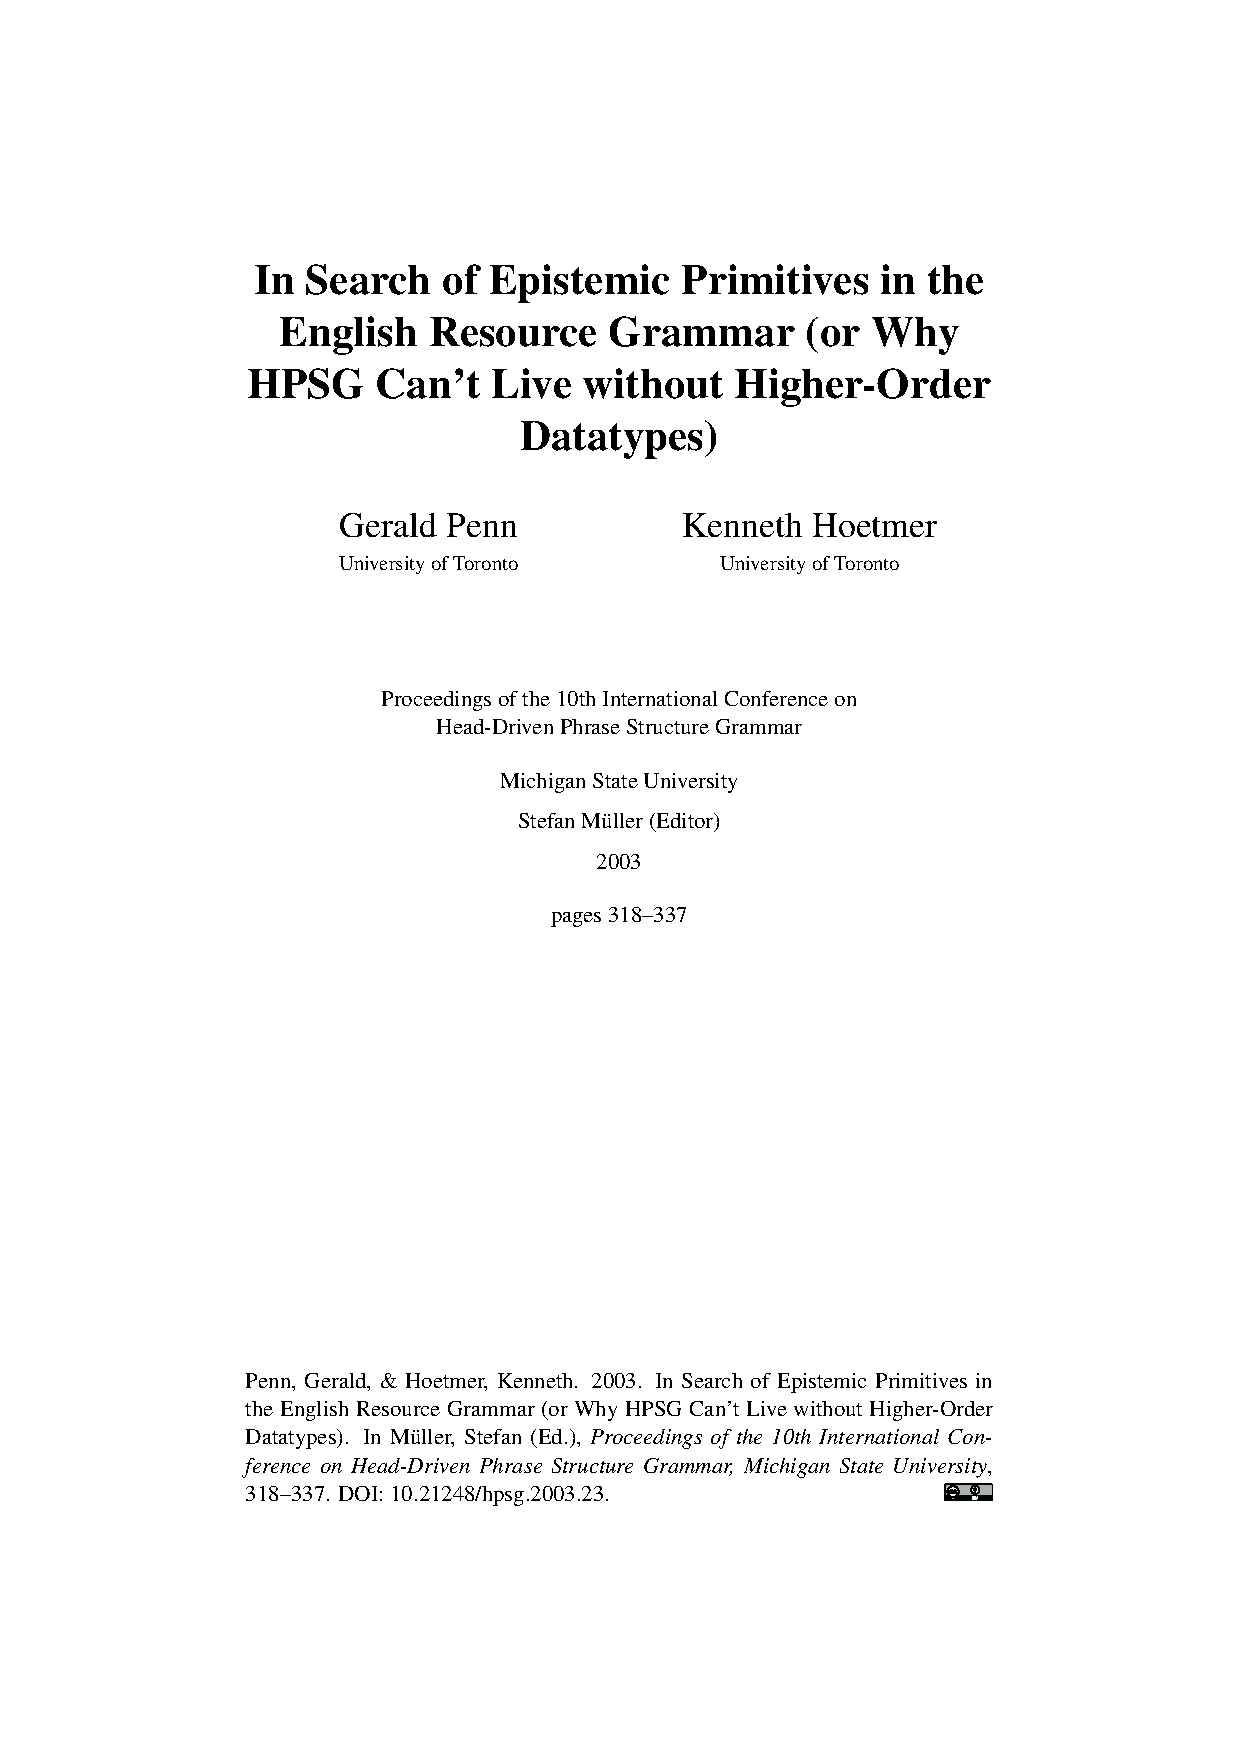
\includepdf[pages=-,pagecommand=\thispagestyle{plain},
            addtotoc={1,section,1,
            {Gerald Penn and Kenneth Hoetmer: In Search of Epistemic Primitives in the English Resource Grammar (or Why HPSG Can't Live without Higher-Order Datatypes)},
             penn-hoetmer}]{penn-hoetmer.pdf}


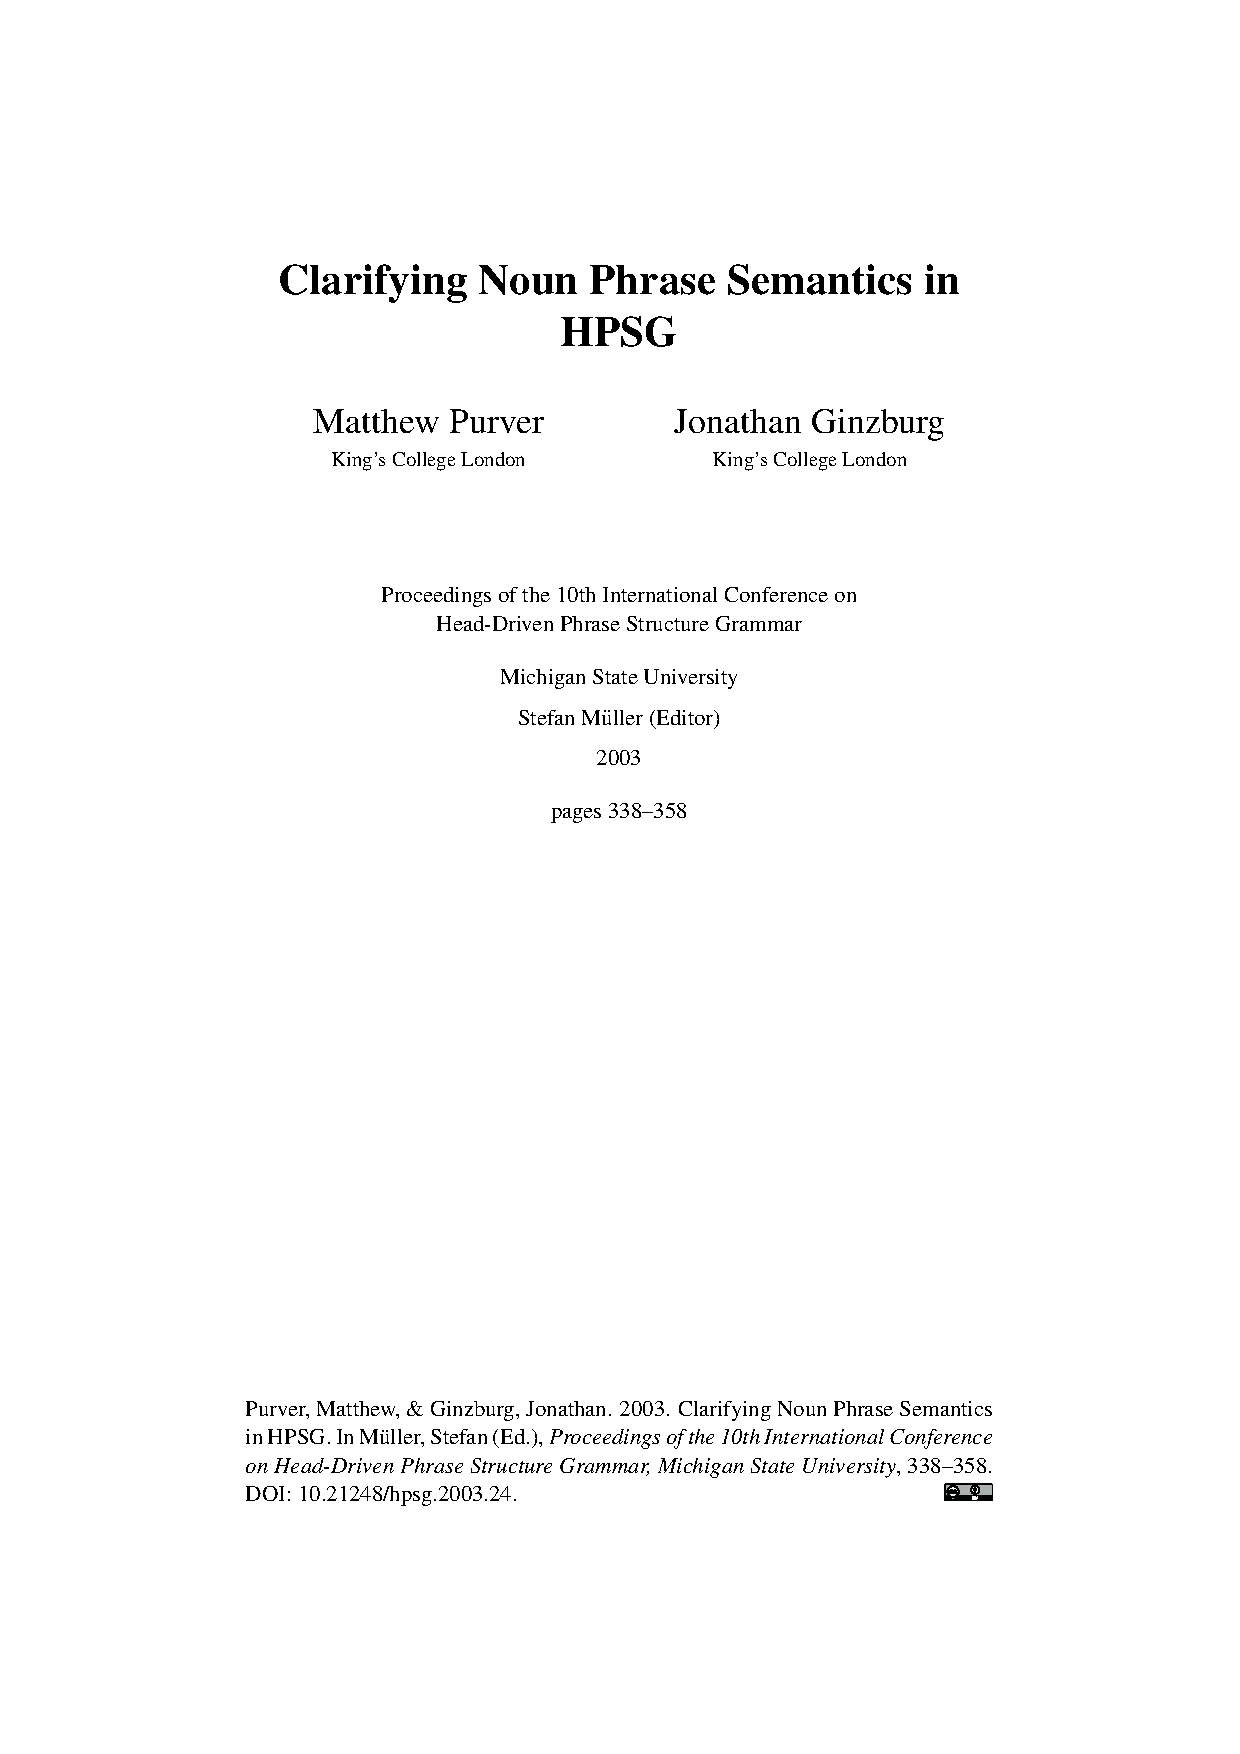
\includepdf[pages=-,pagecommand=\thispagestyle{plain},
            addtotoc={1,section,1,
            {Matthew Purver and Jonathan Ginzburg: Clarifying Noun Phrase Semantics in HPSG},
             purver-ginzburg}]{purver-ginzburg.pdf}


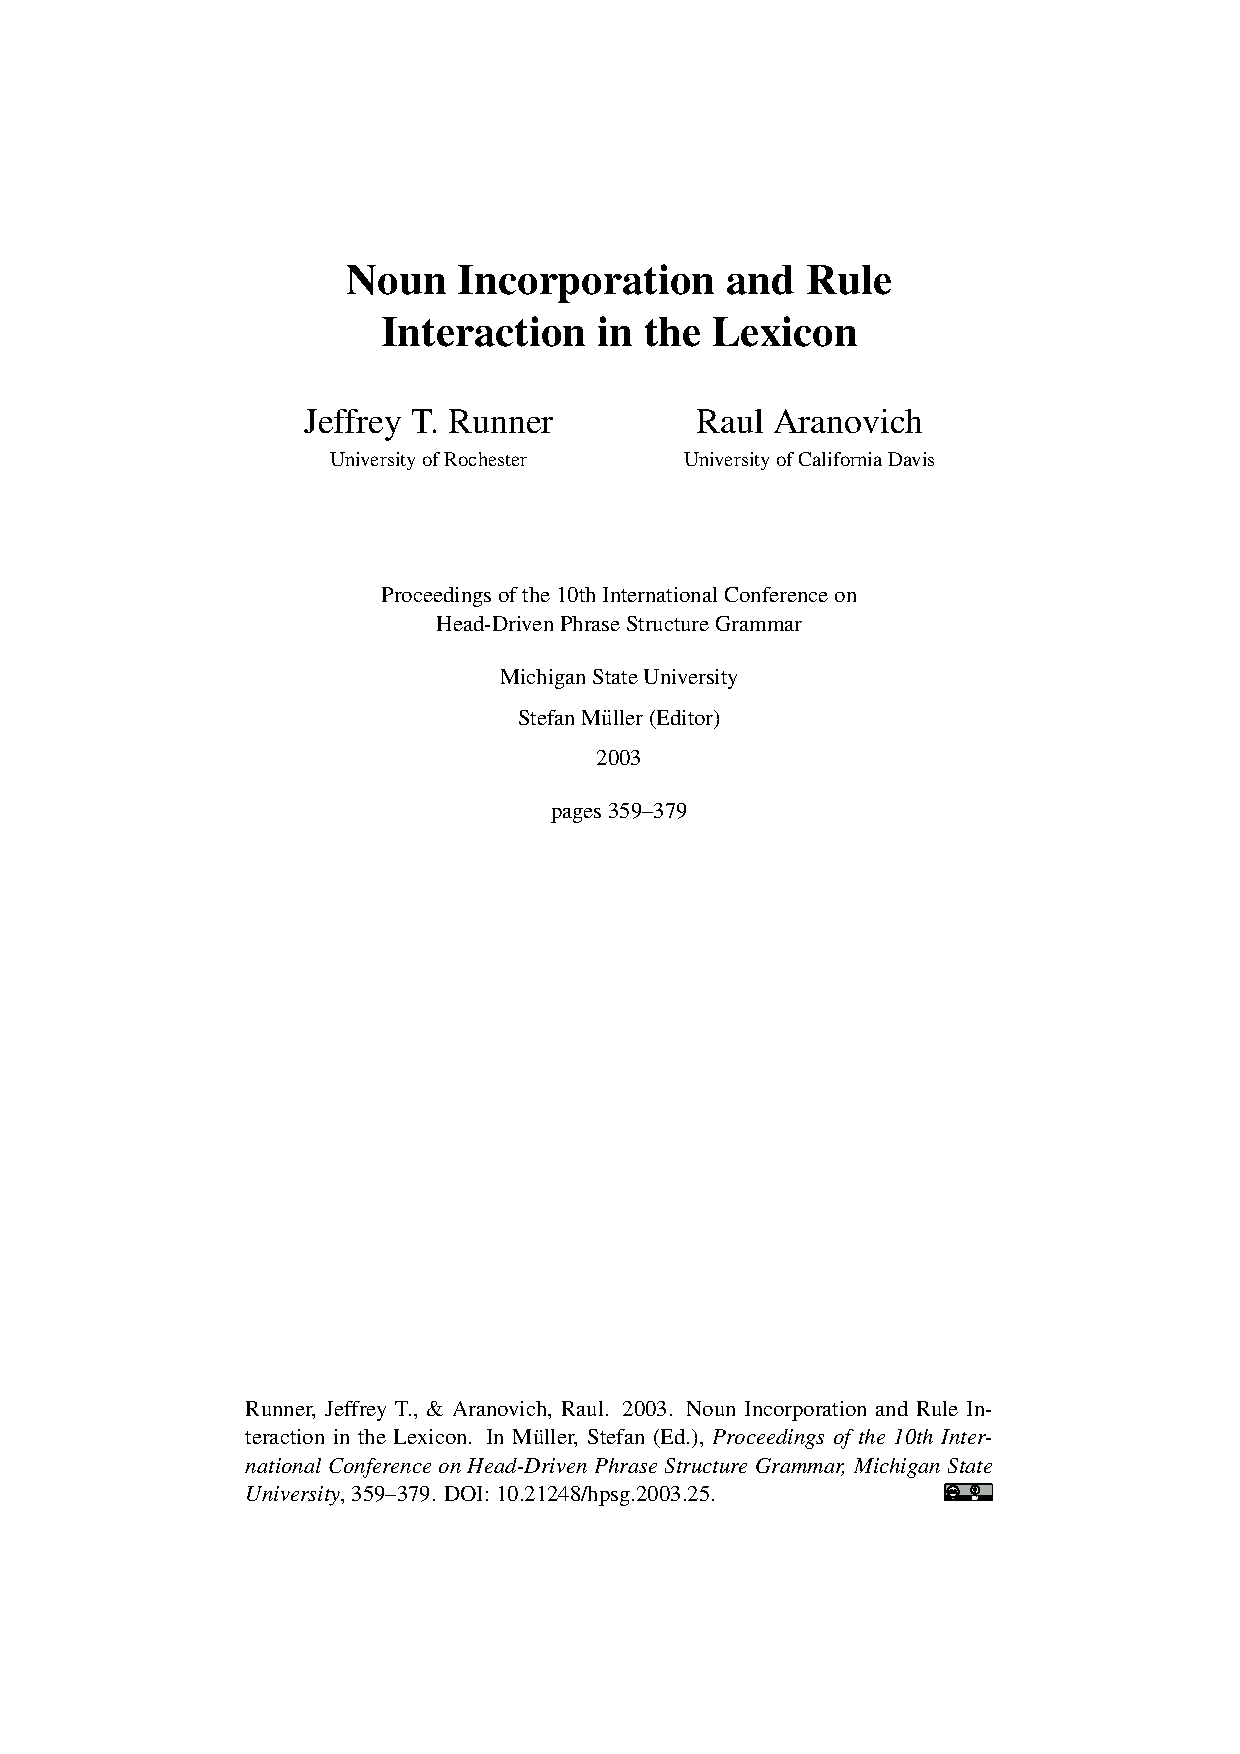
\includepdf[pages=-,pagecommand=\thispagestyle{plain},
            addtotoc={1,section,1,
            {Jeffrey T. Runner and Raul Aranovich: Noun Incorporation and Rule Interaction in the Lexicon},
             runner-aranovich}]{runner-aranovich.pdf}


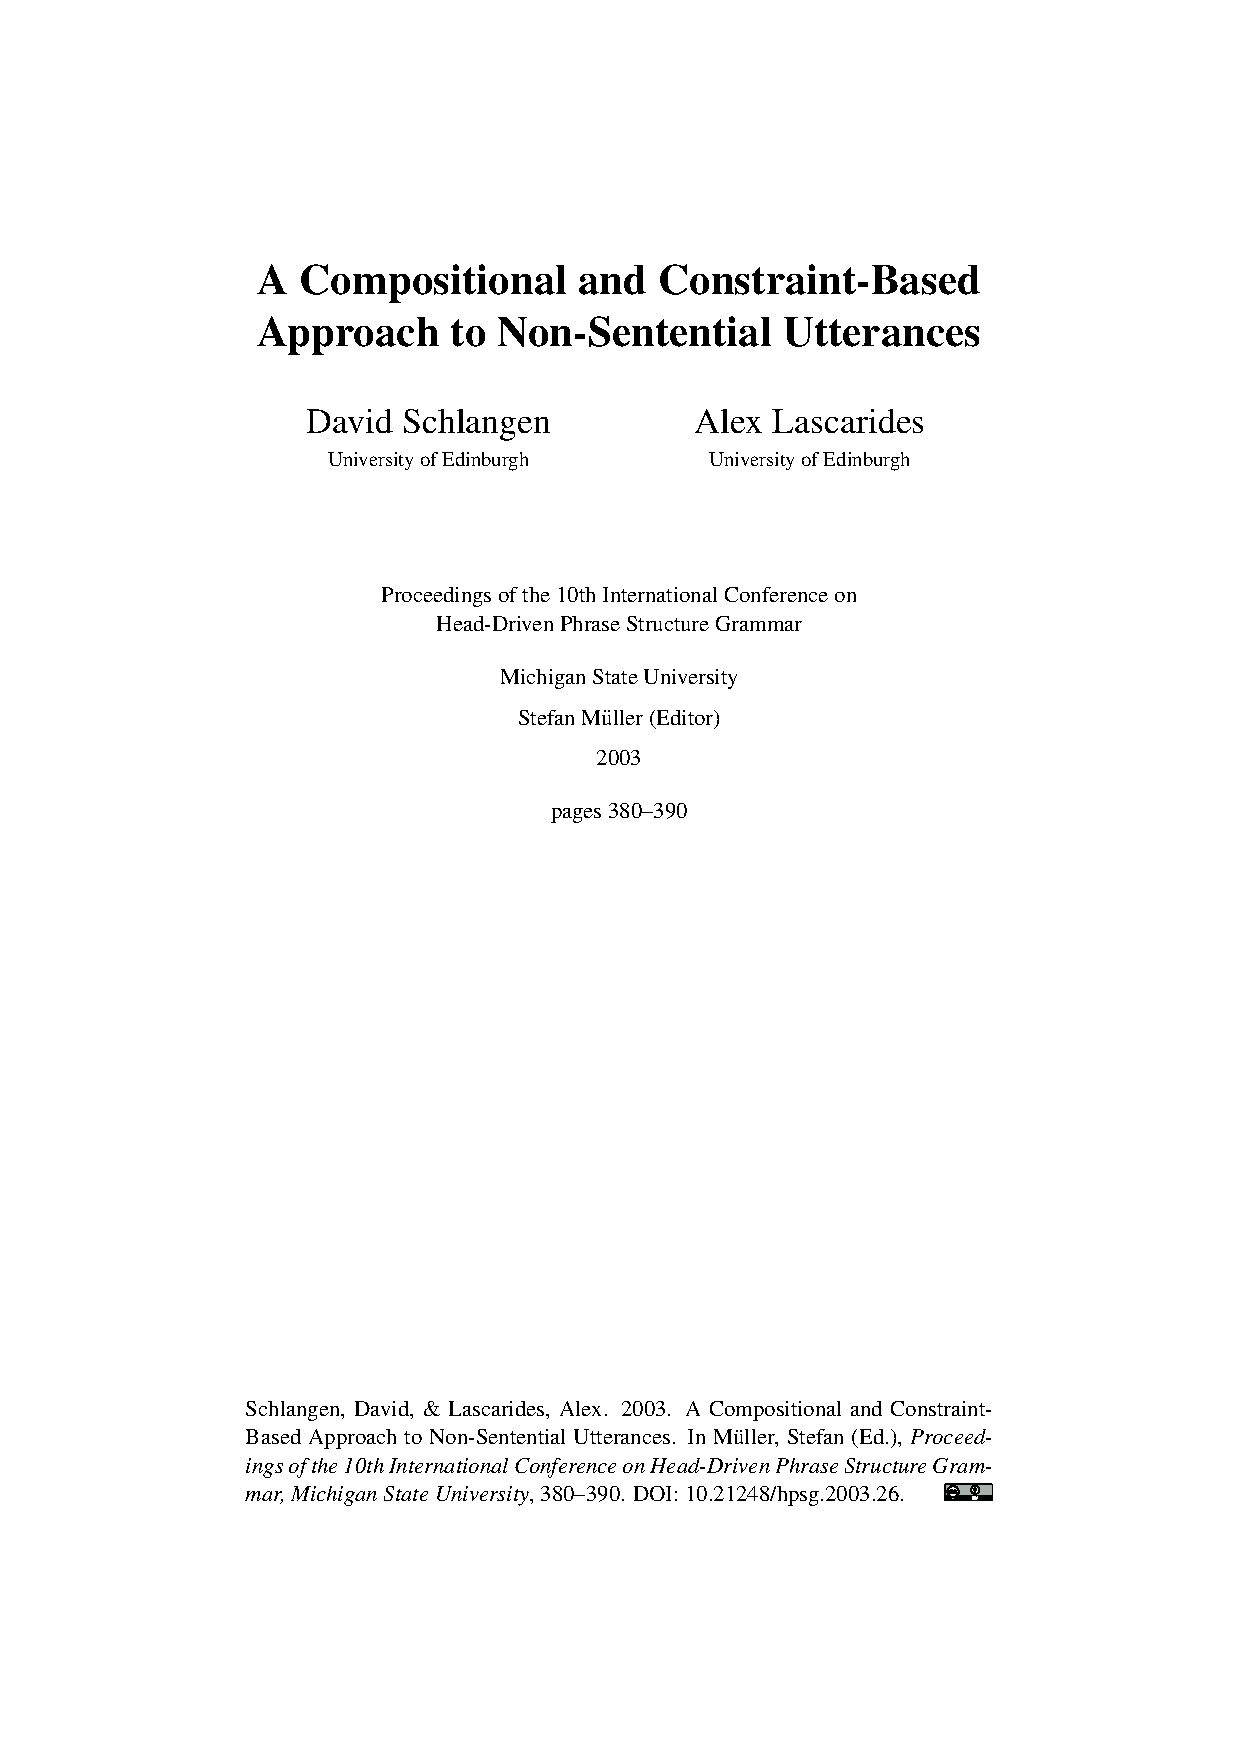
\includepdf[pages=-,pagecommand=\thispagestyle{plain},
            addtotoc={1,section,1,
            {David Schlangen and Alex Lascarides: A Compositional and Constraint-Based Approach to Non-Sentential Utterances},
             schlangen-lascarides}]{schlangen-lascarides.pdf}

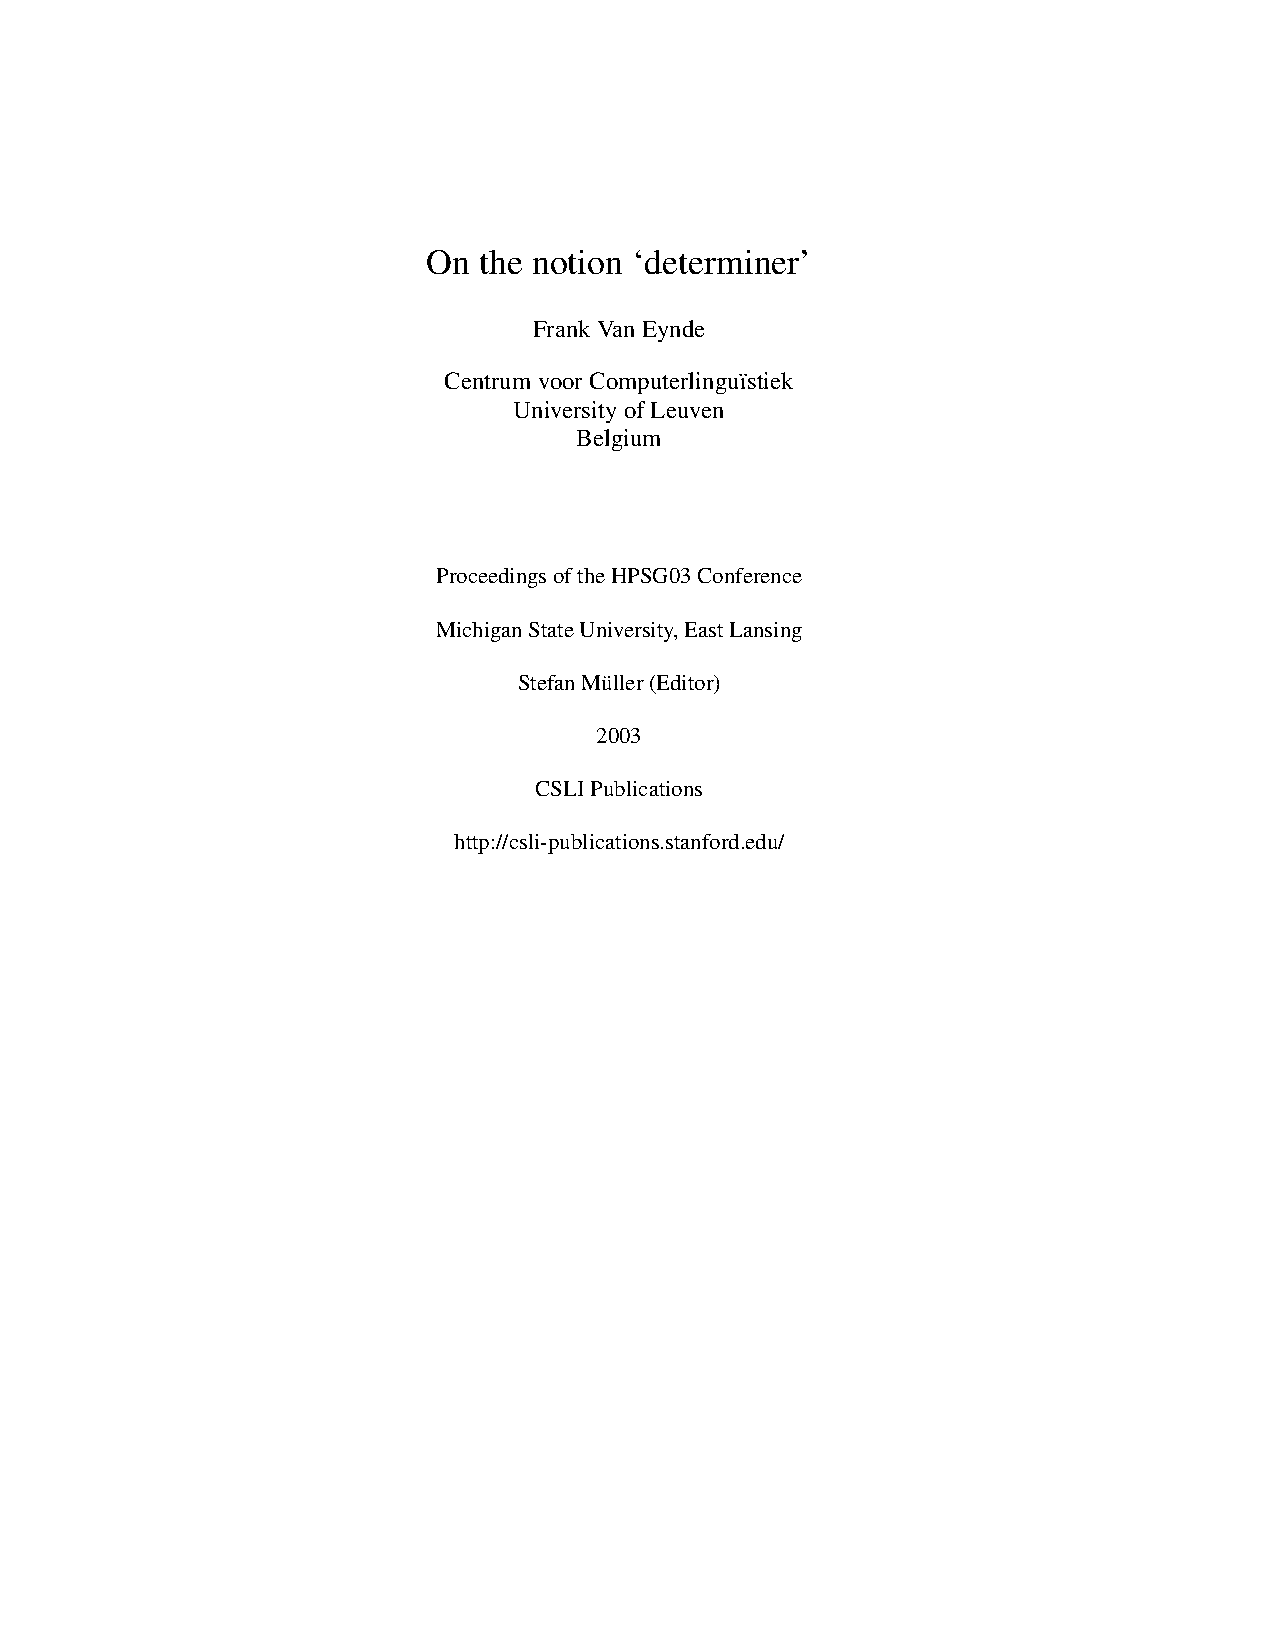
\includepdf[pages=-,pagecommand=\thispagestyle{plain},
            addtotoc={1,section,1,
            {Frank Van Eynde: On the Notion `Determiner'},
             van-eynde}]{van-eynde.pdf}

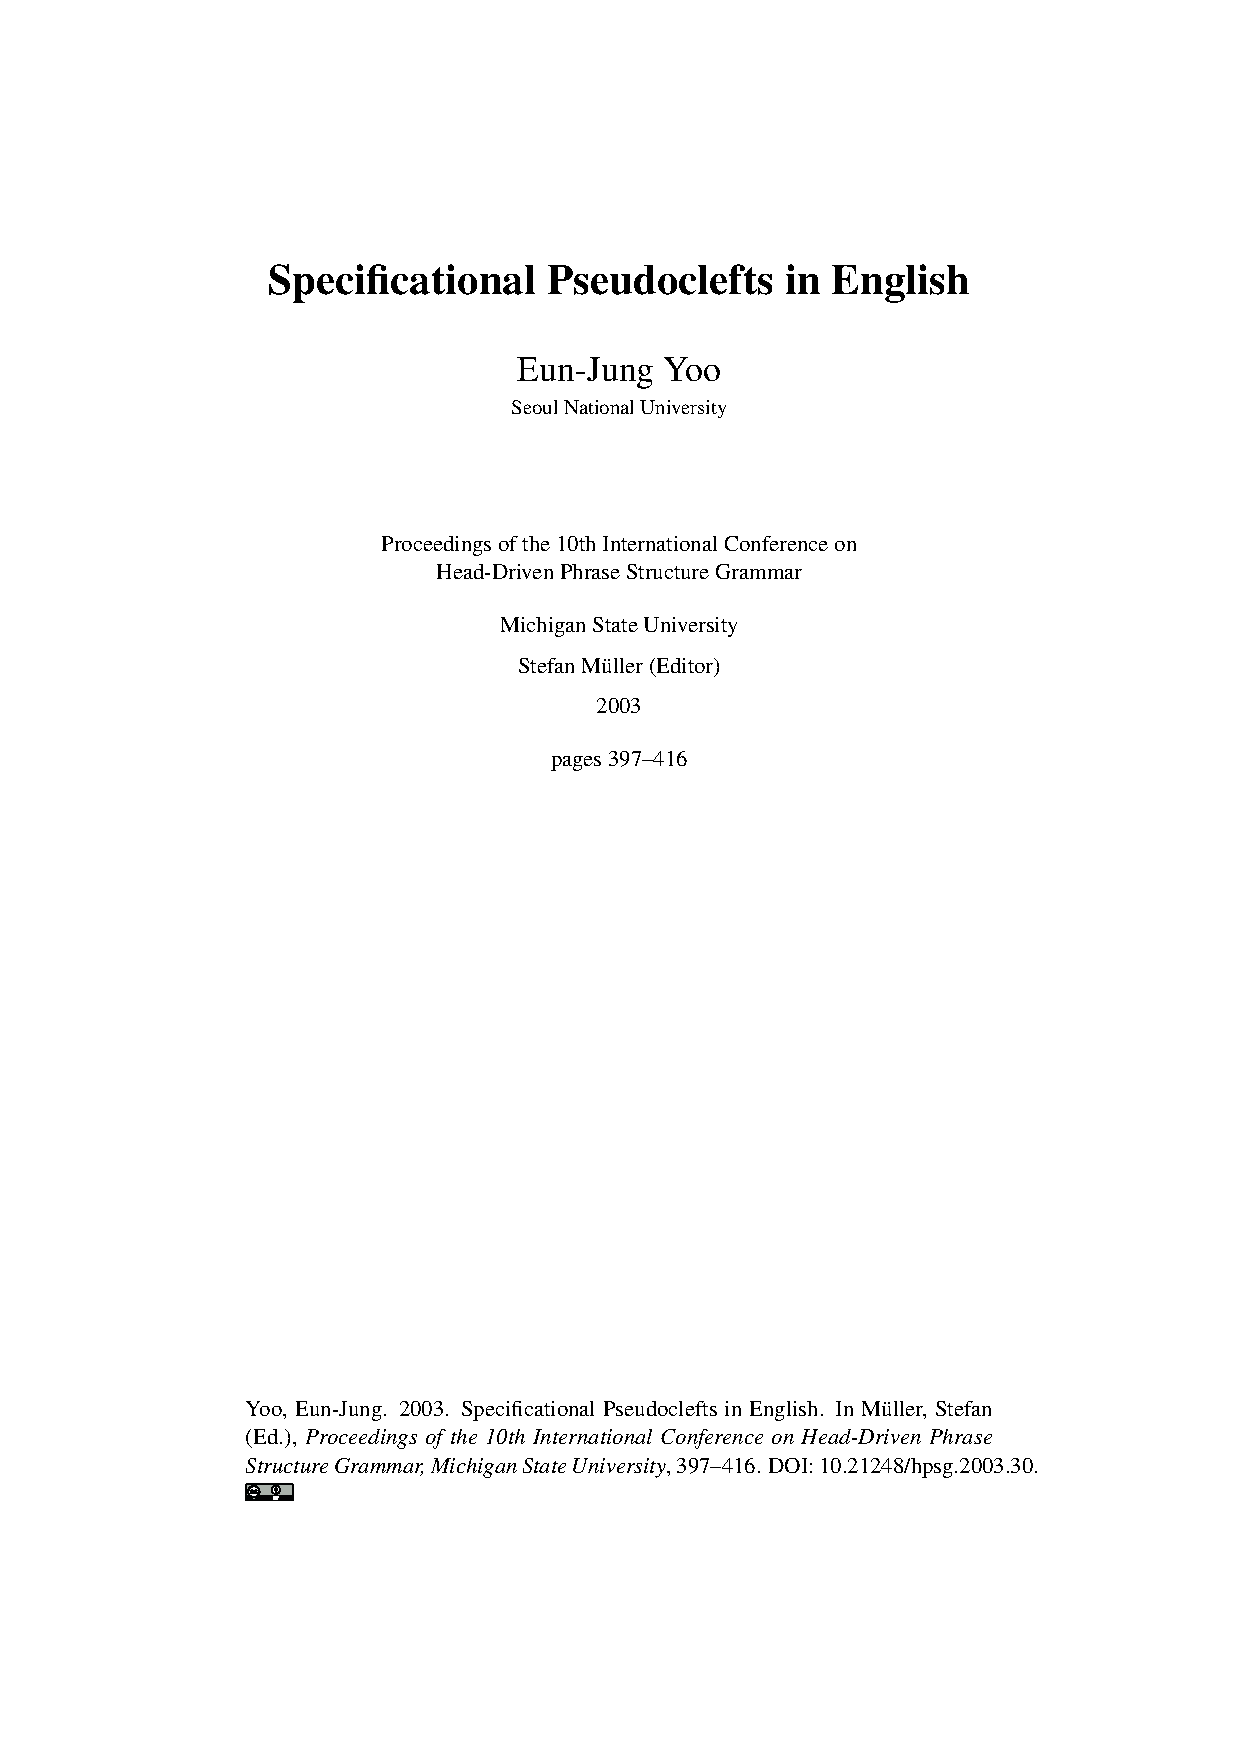
\includepdf[pages=-,pagecommand=\thispagestyle{plain},
            addtotoc={1,section,1,
            {Eun-Jung Yoo: Specificational Pseudoclefts in English},
             yoo}]{yoo.pdf}


\end{document}

